\documentclass{article}

\usepackage[utf8]{inputenc}
\usepackage[T1]{fontenc}
\usepackage{lipsum}
\usepackage{graphicx}
\usepackage{amsmath}
\usepackage[margin=1in]{geometry}
\usepackage{titlesec}
\usepackage{graphicx}
\usepackage{floatflt,epsfig}
\usepackage[utf8]{inputenc}
\usepackage[T1]{fontenc}
\usepackage{lipsum}
\usepackage{graphicx}
\usepackage{amsmath}
\usepackage[margin=1in]{geometry} 
\usepackage{titlesec}
\usepackage{listings}
\usepackage{xcolor}
\usepackage{hyperref}

\hypersetup{
    pdfborder = {0 0 0},
}

\lstdefinelanguage{Java}{
  keywords={abstract,assert,boolean,break,byte,case,catch,char,class,const,continue,default,do,double,else,enum,extends,false,final,finally,float,for,goto,if,implements,import,instanceof,int,interface,long,native,new,null,package,private,protected,public,return,short,static,strictfp,super,switch,synchronized,this,throw,throws,transient,true,try,void,volatile,while},
  morekeywords={[2]System,out},
  morecomment=[l]{//},
  morecomment=[s]{/*}{*/},
  morestring=[b]",
  basicstyle=\small\ttfamily,
  keywordstyle=\color{blue}\bfseries,
  keywordstyle={[2]\color{orange}\bfseries},
  commentstyle=\color{green!70!black},
  stringstyle=\color{red},
  showstringspaces=false,
  tabsize=2,
  breaklines=true,
  breakatwhitespace=true,
  frame=single, 
  captionpos=b
}

\titleformat{\section}
{\LARGE\bfseries}{\thesection}{1em}{}

\titleformat{\subsection}
{\Large\bfseries}{\thesection}{1em}{}

\begin{document}

\pagestyle{empty}


\begin{titlepage} 
    \begin{center}
        {{\Large{\textsc{Alma Mater Studiorum - Università di Bologna}}}}
        \rule[0.1cm]{\textwidth}{0.1px}
        \rule[0.5cm]{\textwidth}{0.6px}\\
        {\large{SCUOLA DI SCIENZE \\ Corso di Laurea in Informatica per il Management}}
    \end{center}
    
    \vspace{90px}
    
    \begin{center}
        {
\includegraphics[width=0.2\textwidth]{logo.png}}\\\vspace*{20pt}
        \LARGE YOUR CITY IS LISTENING TO
    \end{center}
    
    \vspace{100px}
    \par
    \noindent
    \begin{minipage}[t]{0.04\textwidth}
    ~
    \end{minipage}
    \begin{minipage}[t]{0.4\textwidth}
    \end{minipage}
    \hfill
    \begin{minipage}[t]{0.4\textwidth}\raggedleft
        {\fontsize{12}{13}{}\
    \fontsize{12}{13}{\it \\ De Rosa Davide \\ Matricola 1054948 \\ davide.derosa@studio.unibo.it}}
    \end{minipage}
    \begin{minipage}[t]{0.04\textwidth}
    ~
    \end{minipage}
    
    \vspace*{140px}
    
    \begin{center}
        \large{Laboratorio di Applicazioni Mobili}\\
        \large{Anno Accademico 2023/2024}
    \end{center}
    \end{titlepage}
    

\subsection*{Scelte di base}
\large

Per il versionamento dell'app è stato utilizzato \textbf{Git}, con \href{https://github.com/DavideDeRosa/ProgettoLAM}{\underline{\textit{repository}}} accessibile su \textbf{GitHub}.\vspace*{14pt}\\
Per la realizzazione dell'applicativo è stato scelto il linguaggio \textbf{Kotlin}, realizzando un'applicazione in \textbf{Android Nativo}, seguendo il pattern architetturale \textbf{MVVM (Model View ViewModel)}. In questo modo si ottiene una separazione netta tra la \textit{UI} -- ovvero le diverse \textit{View} visibili agli utenti finali -- ed i dati gestiti dal \textit{Model}.\\
Il \textit{ViewModel} permette alle View ed al Model di comunicare e di scambiarsi dati. Alcuni dei vantaggi dell'utilizzo di ViewModel sono:
\begin{enumerate}
    \itemsep0em
    \renewcommand*{\labelenumi}{-}
    \item Se l'activity viene distrutta e ricreata non c'è bisogno di salvare l'\textit{instance state} ogni volta
    \item Permette di avere una separazione netta tra il propretario dei dati (ViewModel) e la logica dell'interfaccia grafica (View)
\end{enumerate}
Tutta l'implementazione di questo pattern architetturale gira attorno all'utilizzo di \textbf{LiveData}. I LiveData sono basati sul concetto di \textbf{Observables}, classi che notificano un cambiamento su dati osservati. Un \textit{Observable} ha una lista nascosta. Ogni volta che un oggetto si \textit{iscrive ai cambiamenti} viene aggiunto a questa lista. Dato ogni cambiamento al dato osservato, tutti i membri della lista vengono notificati richiamando una funzione \textbf{callback}.\vspace*{14pt}\\
Inoltre, i LiveData sono componenti Observable \textit{lifecycle-aware} che notificano solamente gli iscritti in uno stato attivo (\textit{Resumed} o \textit{Started}). Questo è molto utile per activity e fragments, permettendo di osservare dati senza preoccuparsi del loro stato.
\begin{center}
    {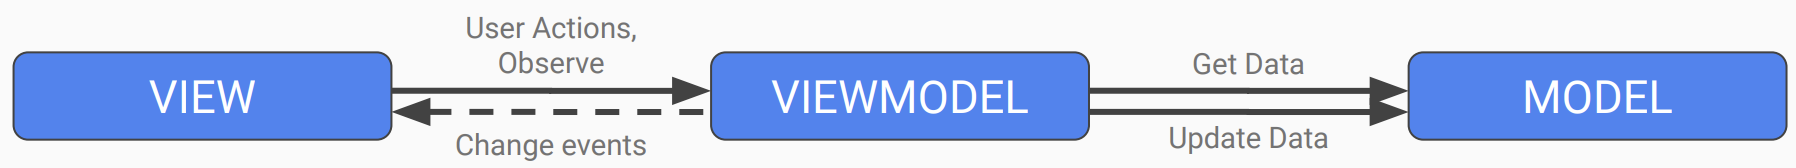
\includegraphics[width=1\textwidth]{mvvm.png}}
\end{center}
Passando alla gestione del \textit{Model}, sono state utilizzate le librerie \textbf{Room} e \textbf{Retrofit}.\vspace*{14pt}\\
\textit{Room} è stata utilizzata per la persistenza dei dati all'interno di un Database Relazionale. Ha permesso di ottenere accesso al database in maniera semplice e veloce.\\
L'utilizzo di Room risulta essere abbastanza intuitivo. Una volta dichiarata una \textit{INSTANCE} del database, basterà creare le diverse tabelle (tramite la creazione di \textbf{Entity}) e il suo corrispettivo \textbf{Dao}, dove verranno dichiarate tutte le funzioni desiderate.\vspace*{14pt}\\
\textit{Retrofit} è stata utilizzata per la gestione delle chiamate API verso il backend. Ha permesso di effettuare chiamate al server in maniera asincrona e di gestire le risposte in maniera efficiente.\\
L'utilizzo di Retrofit è, come per Room, molto intuitivo. Anche in questo caso viene dichiarata una \textit{INSTANCE} di Retrofit, nella quale viene dichiarato l'URL del server dove effettuare le chiamate. Successivamente viene creata un'interfaccia contenente tutte le chiamate desiderate.\vspace*{14pt}\\
Tutte le funzioni inerenti al Database e alle chiamate API vengono gestite all'interno di ViewModel, permettendo un approccio moderno e sicuro.\\
Si osservino ora alcuni esempi, inerenti all'utilizzo di \textit{Room} e \textit{Retrofit} nel contesto dell'applicativo.
\begin{lstlisting}[language = JAVA]
private var fileCorrectlyUploadedLiveData = MutableLiveData<UploadData>()
private var fileCorrectlyUploadedErrorLiveData = MutableLiveData<String>()

fun uploadAudio(token: String, longitude: Double, latitude: Double, audio: MultipartBody.Part) {
    RetrofitInstance.api.uploadAudio(token, longitude, latitude, audio)
        .enqueue(object : Callback<ResponseBody> {
            override fun onResponse(
                call: Call<ResponseBody>,
                response: Response<ResponseBody>
            ) {
                if (response.isSuccessful) {
                    val uploadData =
                        gson.fromJson(
                            response.body()!!.string(),
                            UploadData::class.java
                        )

                    Log.d(
                        "UploadAudio 200",
                        "UploadAudio 200: " + uploadData.toString()
                    )

                    fileCorrectlyUploadedLiveData.value = uploadData
                } else {
                    when (response.code()) {
                        401 -> {
                            val userNotAuthorized = gson.fromJson(
                                response.errorBody()!!.string(),
                                UserNotAuthorized::class.java
                            )

                            Log.d(
                                "UploadAudio 401",
                                "UploadAudio 401 User Not Authorized: " + userNotAuthorized.detail
                            )

                            fileCorrectlyUploadedErrorLiveData.value = userNotAuthorized.detail
                        }

                        413 -> {
                            val fileTooBig = gson.fromJson(
                                response.errorBody()!!.string(),
                                FileTooBig::class.java
                            )

                            Log.d(
                                "UploadAudio 413",
                                "UploadAudio 413 File too big: " + fileTooBig.detail
                            )

                            fileCorrectlyUploadedErrorLiveData.value = fileTooBig.detail
                        }

                        415 -> {
                            val fileNotAudio = gson.fromJson(
                                response.errorBody()!!.string(),
                                FileNotAudio::class.java
                            )

                            Log.d(
                                "UploadAudio 415",
                                "UploadAudio 415 File not audio: " + fileNotAudio.detail
                            )

                            fileCorrectlyUploadedErrorLiveData.value = fileNotAudio.detail
                        }
                    }
                }
            }

            override fun onFailure(call: Call<ResponseBody>, t: Throwable) {
                Log.d("Fail Upload Audio", t.message.toString())

                fileCorrectlyUploadedErrorLiveData.value = t.message
            }
        })
}

fun observeFileCorrectlyUploadedLiveData(): LiveData<UploadData> {
    return fileCorrectlyUploadedLiveData
}

fun observeFileCorrectlyUploadedErrorLiveData(): LiveData<String> {
    return fileCorrectlyUploadedErrorLiveData
}
\end{lstlisting}
Il seguente blocco di codice rappresenta un esempio di chiamata API eseguita tramite Retrofit, nello specifico la chiamata inerente all'\textit{upload dell'audio}.\\
Come si può notare, il tutto è gestito tramite l'utilizzo di \textit{LiveData} -- in questo caso due: uno per l'esito positivo, l'altro per quello negativo -- il quale ci permette di gestire al meglio le chiamate asincrone effettuate da Retrofit.
\begin{lstlisting}[language = JAVA]
private fun observeUpload() {
    audioViewModel.observeFileCorrectlyUploadedLiveData().observe(this) {
        Toast.makeText(this, "Caricamento avvenuto con successo!", Toast.LENGTH_SHORT).show()

        audioViewModel.insertAudioDb(
            AudioDataEntity(
                username = DataSingleton.username,
                longitude = longitude,
                latitude = latitude,
                locationName = getLocationName(longitude, latitude),
                bpm = it.bpm,
                danceability = it.danceability,
                loudness = it.loudness,
                genre = it.genre.getMaxGenre().first,
                mood = it.mood.getMaxMood().first,
                instrument = it.instrument.getMaxInstrument().first
            )
        )

        goToAppActivity()
    }

    audioViewModel.observeFileCorrectlyUploadedErrorLiveData().observe(this) {
        Toast.makeText(this, it, Toast.LENGTH_SHORT).show()
        deleteRecording()
        goToLogin()
    }
}
\end{lstlisting}
Ovunque si voglia utilizzare la funzione \textit{uploadAudio(\dots)} sarà necessario \textbf{osservare} i due LiveData inerenti, implementando tutta la logica all'interno del blocco di codice eseguito una volta ricevuto il LiveData aggiornato (come si può notare nel blocco di codice).\vspace*{14pt}\\
Per completezza, ecco anche un esempio di utilizzo di \textit{Room}.
\begin{lstlisting}[language = JAVA]
private lateinit var audioDbLiveData: LiveData<AudioDataEntity>

fun getAudioById(id: Int) {
    audioDbLiveData = audioDatabase.audioDataDao().getAudioById(id)
}

fun observeAudioDbLiveData(): LiveData<AudioDataEntity> {
    return audioDbLiveData
}
\end{lstlisting}
il quale richiama il seguente metodo presente nel \textbf{Dao}:
\begin{lstlisting}[language = JAVA]
@Query("SELECT * FROM audiodata WHERE id = :id")
fun getAudioById(id: Int): LiveData<AudioDataEntity>
\end{lstlisting}
Anche in questo caso viene seguita la logica di osservare i LiveData, permettendo una gestione asincrona delle chiamate e di gestione delle risposte.\vspace*{14pt}\\
Per concludere le diverse scelte di base, segnalo anche l'utilizzo delle \textbf{Shared Preferences}.\\
Quest'ultime sono state utilizzate per diversi controlli, come quello per la connessione ad Internet e per la gestione dell'account all'interno dell'app.\vspace*{14pt}\\
Per non dover accedere ad ogni avvio dell'app, vengono utilizzate le shared preferences per mantenere persistenti \textit{token} ed \textit{username} ad ogni avvio.\\
Nel momento in cui avviene un logout, o il token risulta essere non valido, vengono resettate.

\pagebreak

\subsection*{Implementazione}
\large
\textit{Login e Registrazione}\\
\begin{minipage}[t]{0.6\textwidth}
    \raggedright
    \vspace*{10pt}
    All'avvio dell'app, la prima \textit{Activity} mostrata è quella inerente al \textbf{Login} dell'account. Prima di mostrare la schermata visibile in foto, viene effettuato un controllo di connessione ad Internet. Se non è presente alcuna connessione, si verrà reindirizzati ad una sezione \textbf{Offline}, con funzionalità limitate (se ne parlerà successivamente).\\
    In caso di connessione attiva, si può procedere all'accesso. Un ulteriore controllo viene effettuato in caso di presenza di accesso già effettuato. Se il \textit{Token} risulta essere ancora valido, non sarà necessario effettuare il Login, ma si verrà reindirizzati direttamente alla schermata principale dell'app.\\
    Inoltre, all'avvio dell'app viene richiesto il permesso per ricevere notifiche, necessario per la funzionalità di \textit{upload in background} (se ne parlerà successivamente).
\end{minipage}
\hfill
\begin{minipage}[t]{0.35\textwidth}
    \centering
    \vspace*{0pt}
    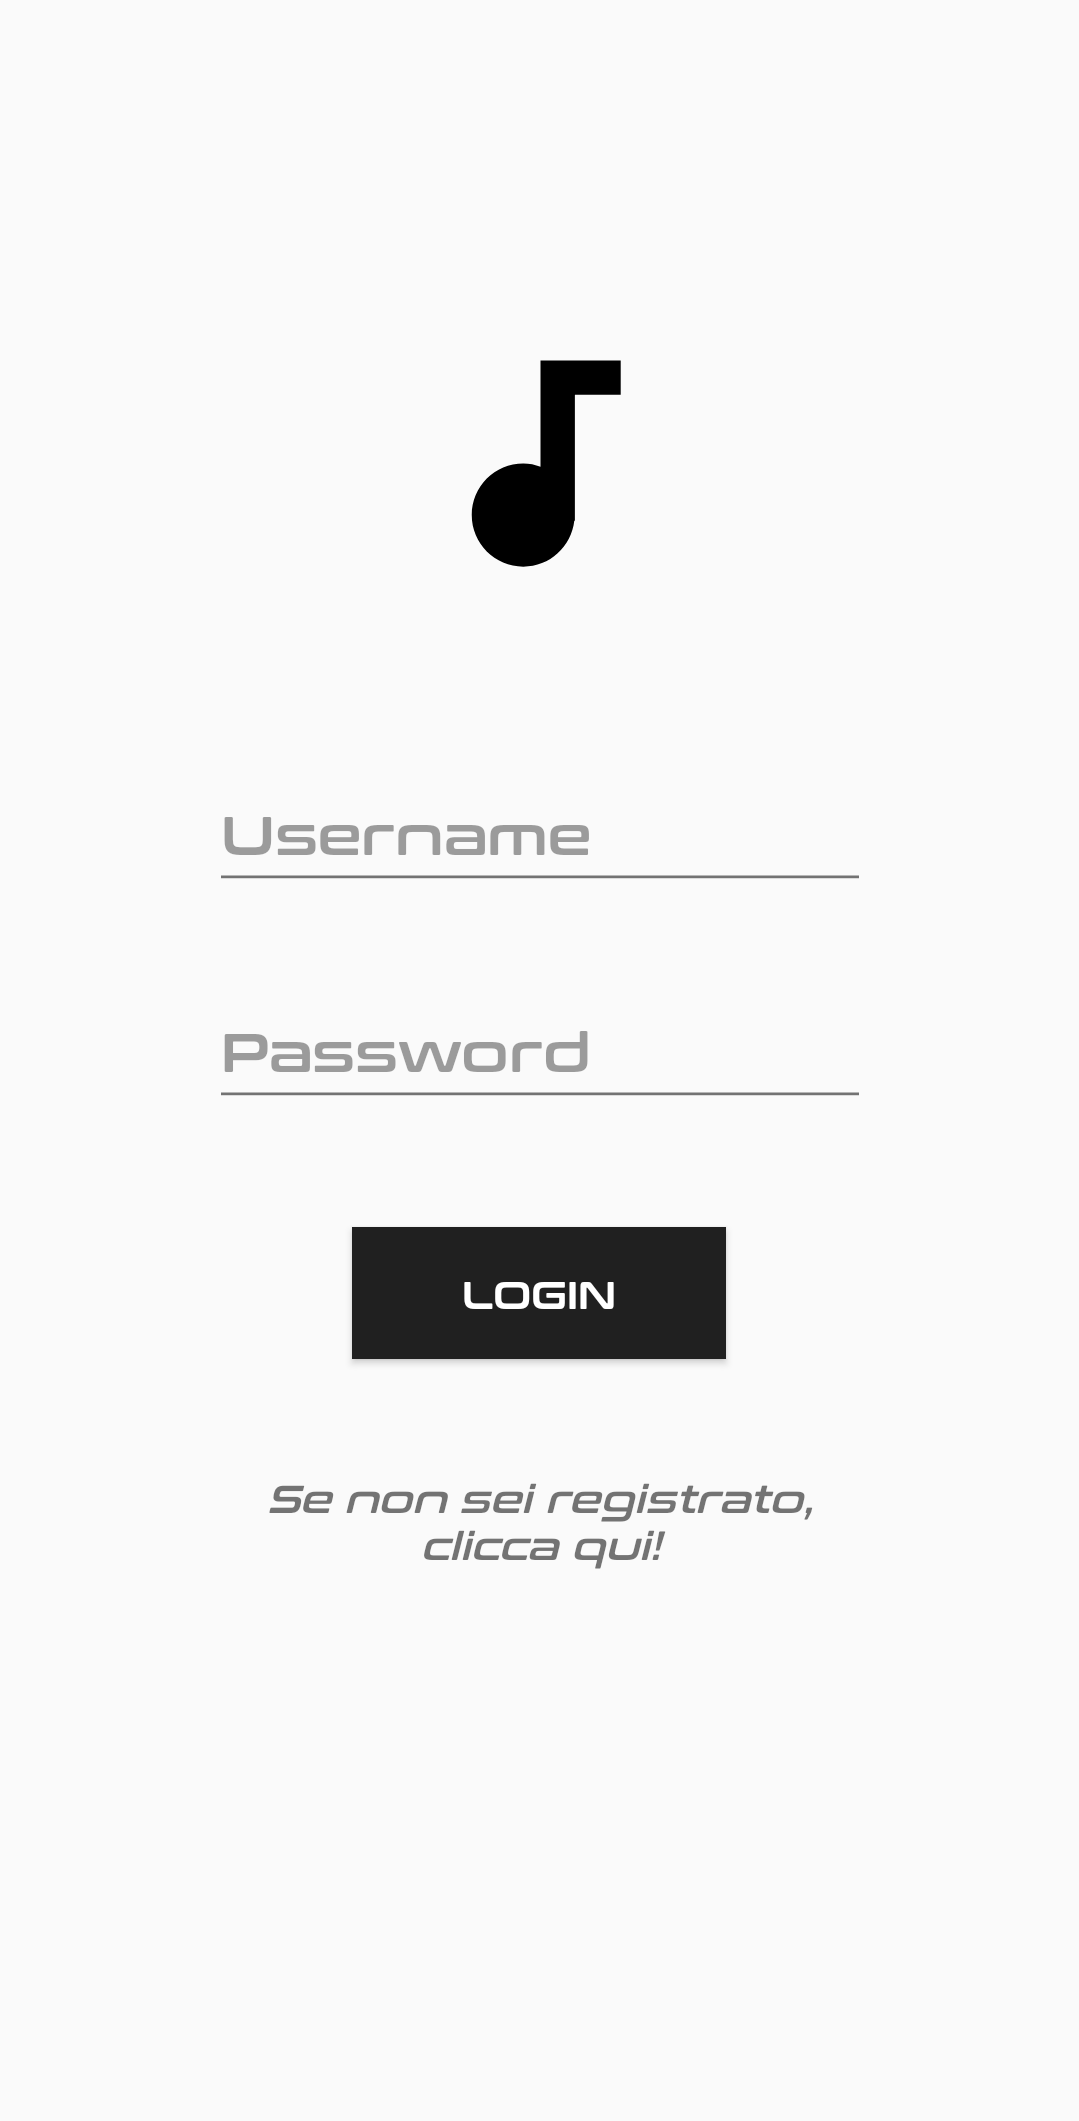
\includegraphics[width=0.8\textwidth]{login.png}\vspace*{40pt}
\end{minipage}
\begin{minipage}[t]{0.35\textwidth}
    \centering
    \vspace*{0pt}
    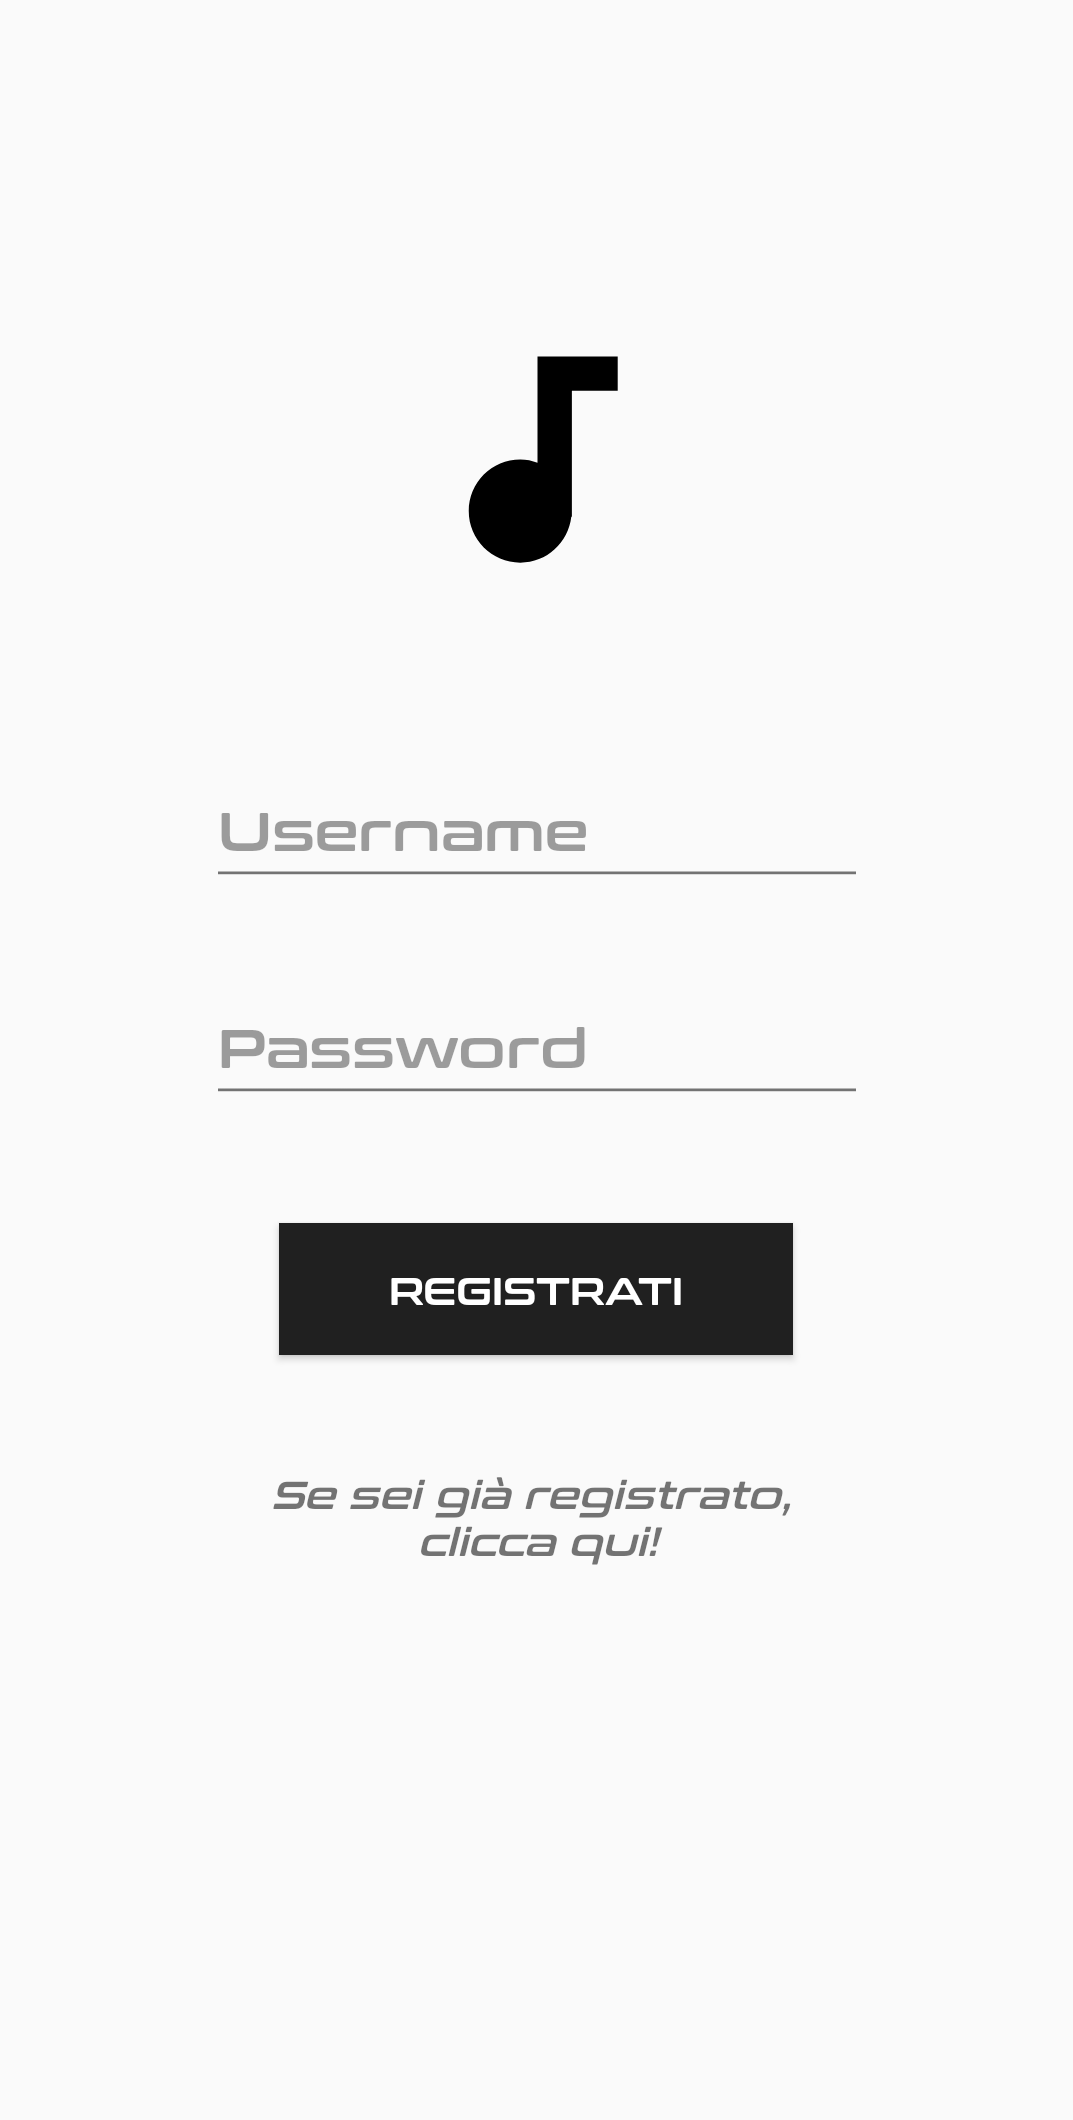
\includegraphics[width=0.8\textwidth]{registrazione.png}
\end{minipage}
\hfill
\begin{minipage}[t]{0.6\textwidth}
    \raggedright
    \vspace*{10pt}
    Per quanto riguarda la \textbf{Registrazione}, è possibile registrarsi tramite un'Activity molto simile a quella del Login.\\
    In questo caso, una volta registrati con successo si verrà reindirizzati alla schermata di Login, per effettuare l'accesso.\\
    In caso di account già esistente, verrà notificato l'errore.
\end{minipage}

\quad \vspace*{30pt}\\
\textit{Audio Personali}\\
\begin{minipage}[t]{0.6\textwidth}
    \raggedright
    \vspace*{10pt}
    La seguente Activity presenta una \textbf{Navigation Bottom Bar}, la quale permette di selezionare tre diversi \textbf{Fragment}.\vspace*{14pt}\\
    Il primo di questi è quello inerente agli \textbf{Audio Personali}. In questa schermata sono presenti tutti gli audio caricati dall'utente. Gli audio sono visualizzati tramite una \textbf{Recycler View}, caricata dinamicamente attraverso la chiamata API \textit{"audio/my"}.\\
    Per ogni audio caricato sul server, vengono salvati all'interno del database locale tutti i suoi metadati, permettendone una visualizzazione anche Offline (se ne parlerà successivamente).
\end{minipage}
\hfill
\begin{minipage}[t]{0.35\textwidth}
    \centering
    \vspace*{0pt}
    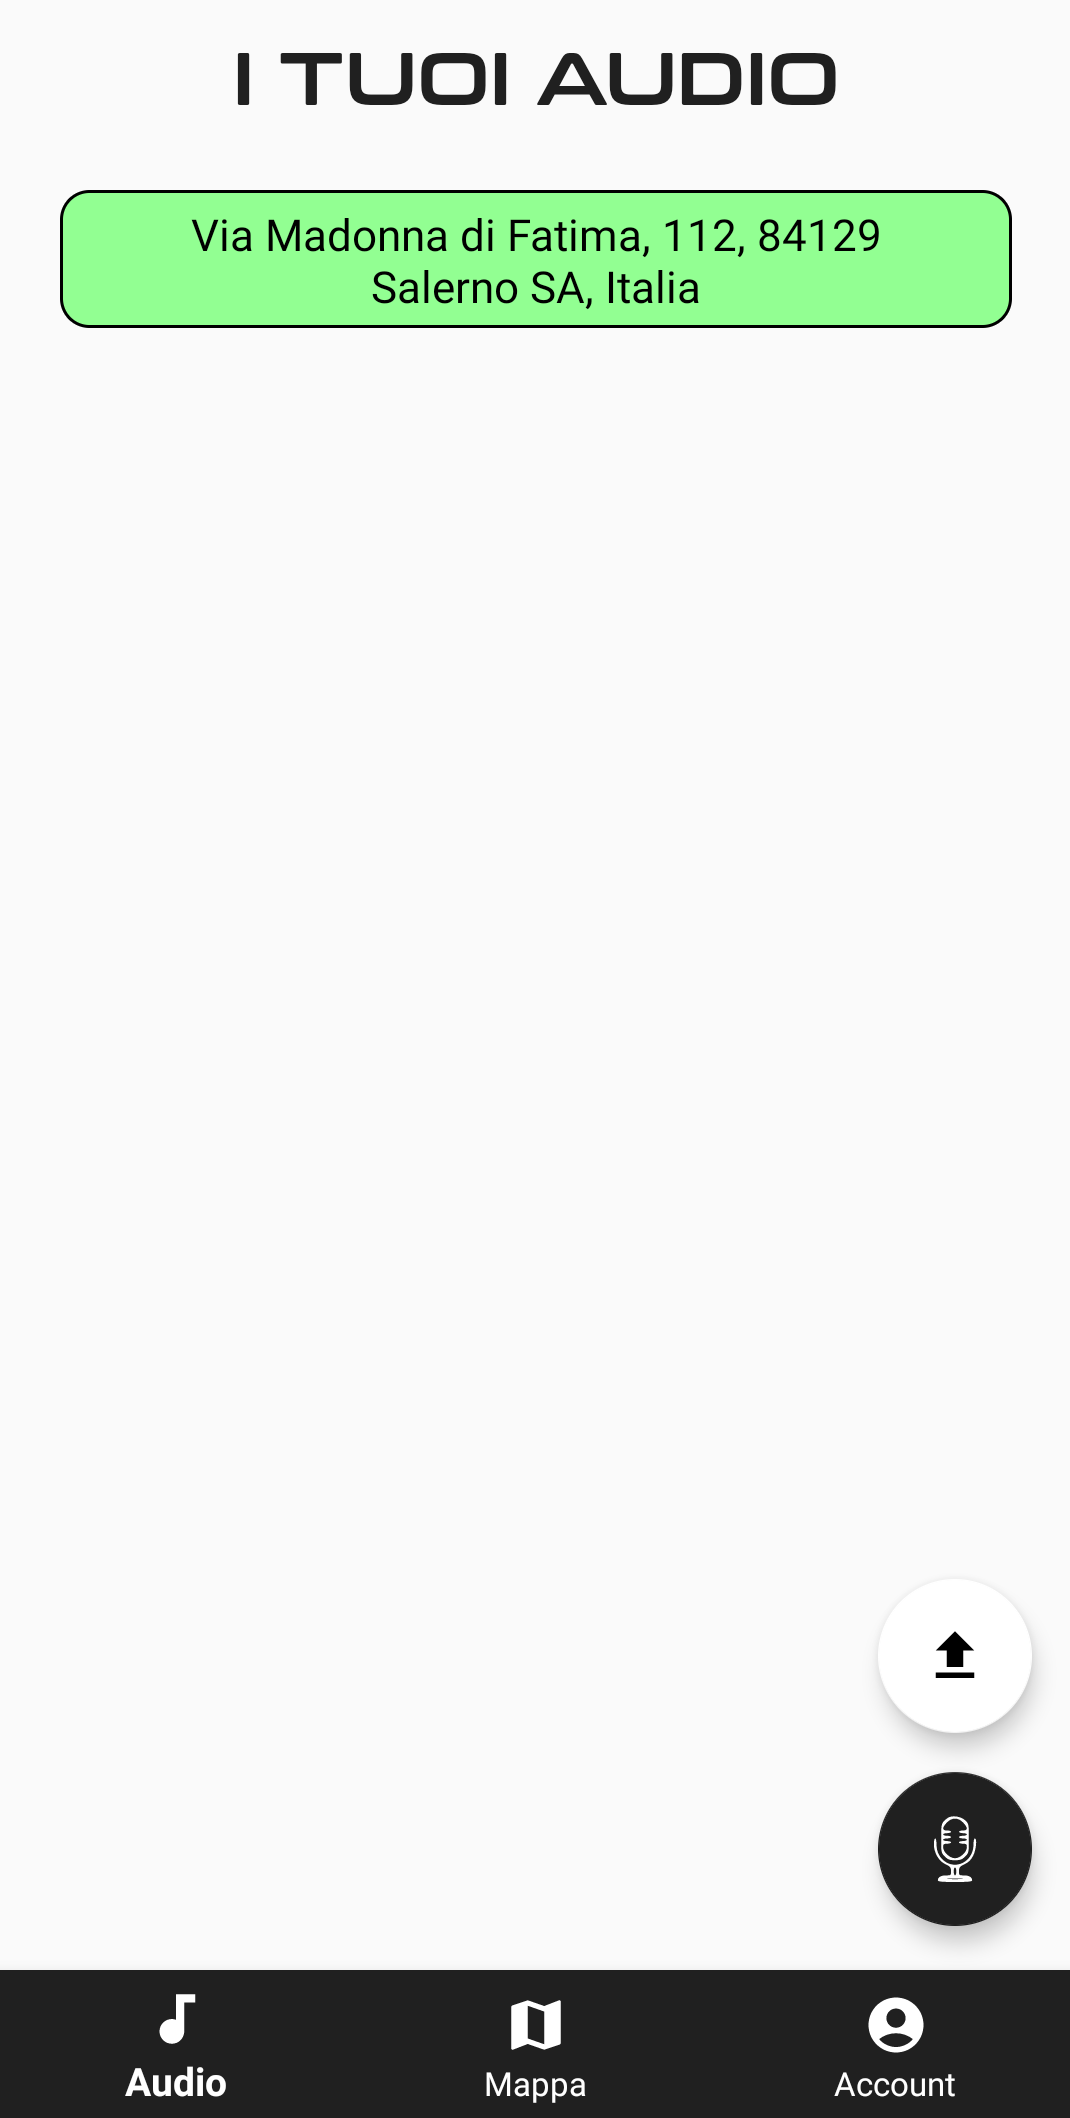
\includegraphics[width=0.8\textwidth]{audiopersonali.png}\vspace*{40pt}
\end{minipage}
\begin{minipage}[t]{0.35\textwidth}
    \centering
    \vspace*{0pt}
    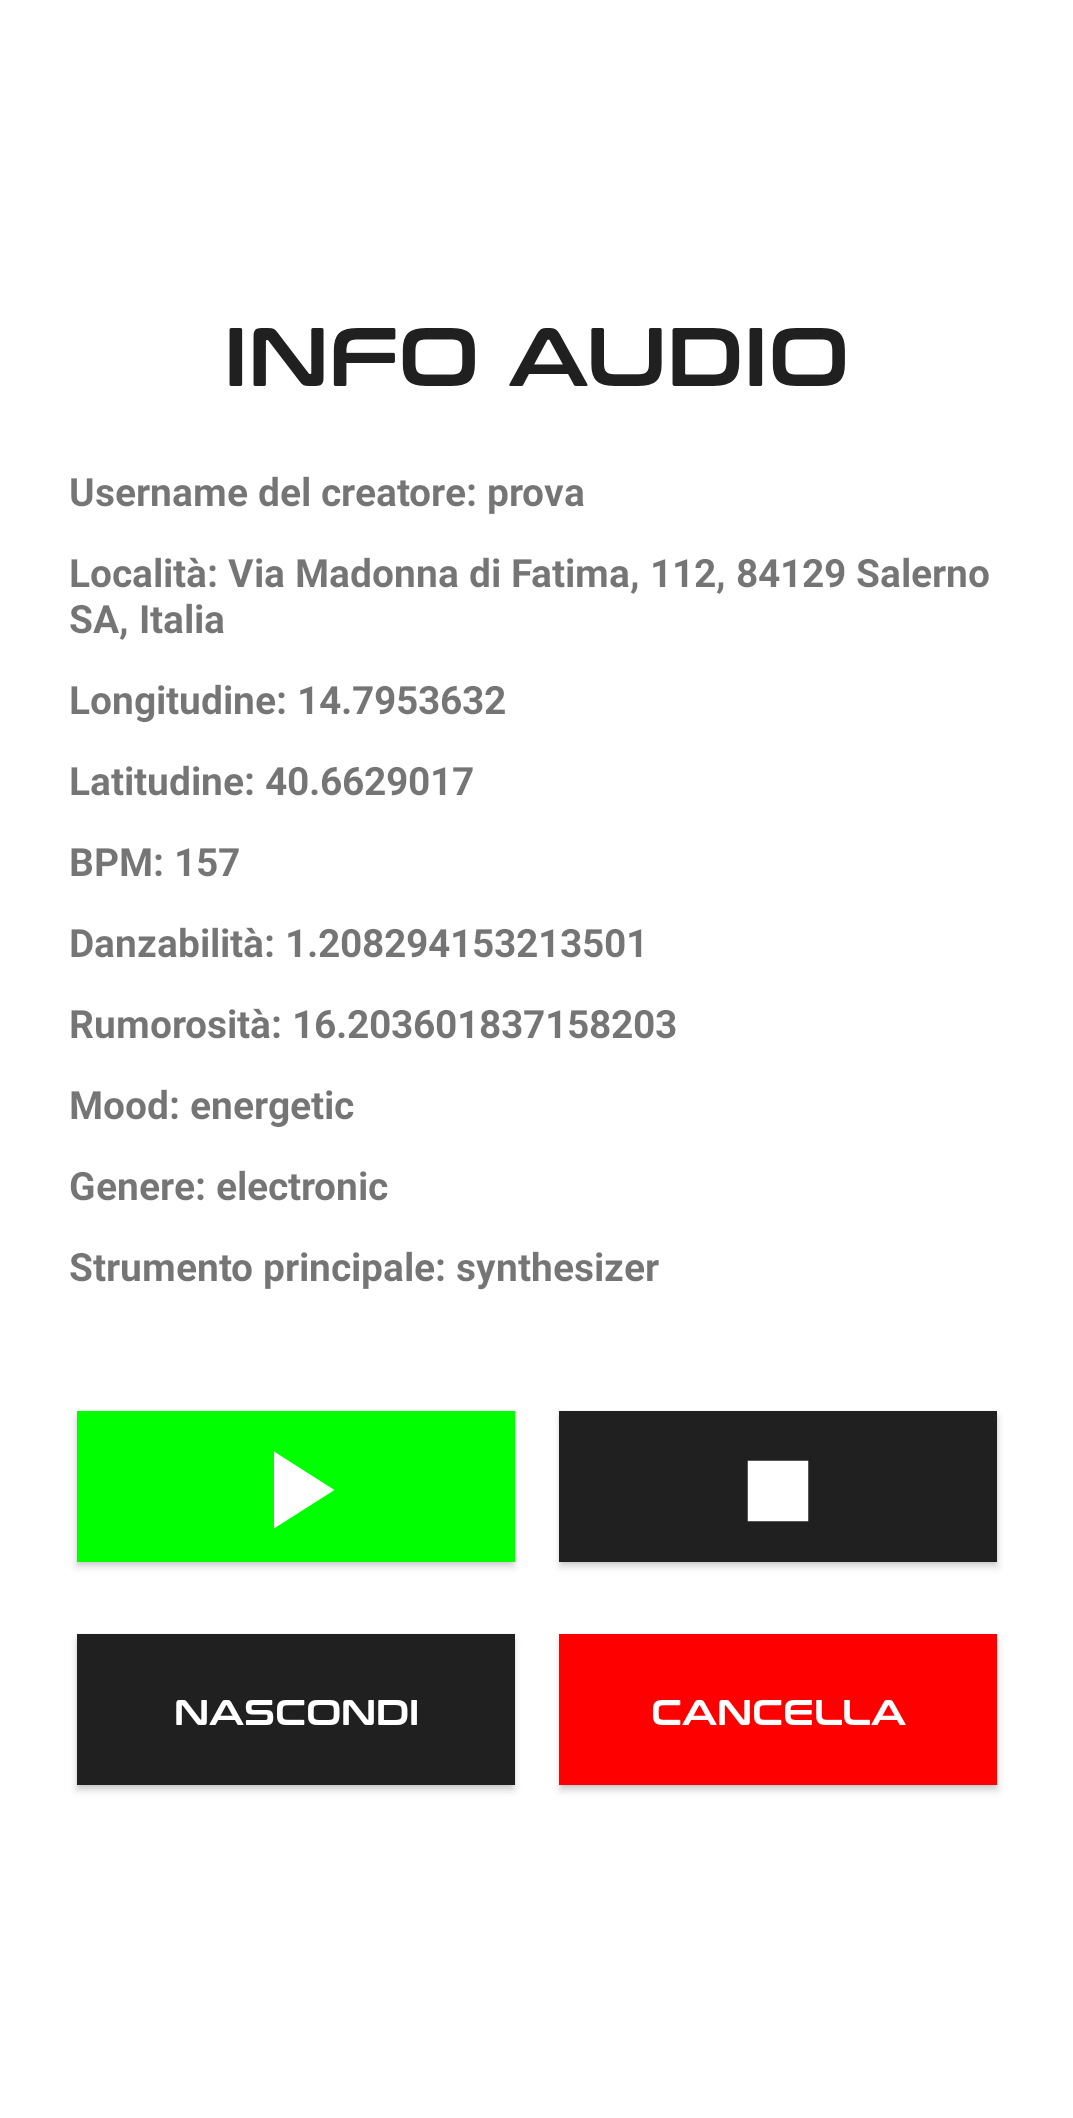
\includegraphics[width=0.8\textwidth]{myaudiodata.png}
\end{minipage}
\hfill
\begin{minipage}[t]{0.6\textwidth}
    \raggedright
    \vspace*{40pt}
    Una volta cliccato uno degli elementi nella lista, si verrà reindirizzati alla seguente Activity, dove vengono mostrati tutti i metadati inerenti all'audio caricato.\\
    E' stato inoltre implementato un controllo che verifica la presenza dei metadati in locale una volta cliccato l'elemento. Se non è presente, verrà chiamata l'API \textit{"audio/\{id\}"} per ottenere i suoi metadati e salvarli in locale.\\
    Sarà quindi possibile \textbf{ascoltare la registrazione} caricata in precedenza.\\
    Inoltre, è possibile \textbf{nascondere} l'audio dalla piattaforma, o \textbf{cancellarlo} definitivamente.
\end{minipage}

\quad \vspace*{60pt}\\
\textit{Registrazione Audio e Lista Upload}\\
\begin{minipage}[t]{0.6\textwidth}
    \raggedright
    \vspace*{10pt}
    Premendo sul \textbf{Floating Button} nero presente nel Fragment degli Audio Personali si verrà reindirizzati all'Activity per la \textbf{registrazione di un nuovo audio}.\\
    Inizialmente, è presente solo il bottone \textit{Ottieni Localizzazione}, il quale richiede i permessi di localizzazione. Una volta geolocalizzato l'audio, diventa visibile la località con i pulsanti \textit{Avvia Registrazione} ed \textit{Importa Registrazione} (se ne parlerà successivamente nella sezione Extra).\\
    Una volta avviata la registrazione, diventano visibili la durata della registrazione e il bottone \textit{Interrompi Registrazione}. Premuto l'ultimo, verranno mostrati tutti gli altri bottoni.\\
    Si potrà \textbf{riascoltare} l'audio appena registrato, \textbf{cancellarlo}, o \textbf{confermarlo} effettuando il caricamento. Prima di procedere al caricamento, viene controllata la presenza di una connessione Wi-Fi. Se non presente, verrà richiesto se si vuole comunque procedere con i dati mobili. In caso contrario, l'audio verrà salvato in locale nel database per poter essere caricato successivamente.
\end{minipage}
\hfill
\begin{minipage}[t]{0.35\textwidth}
    \centering
    \vspace*{10pt}
    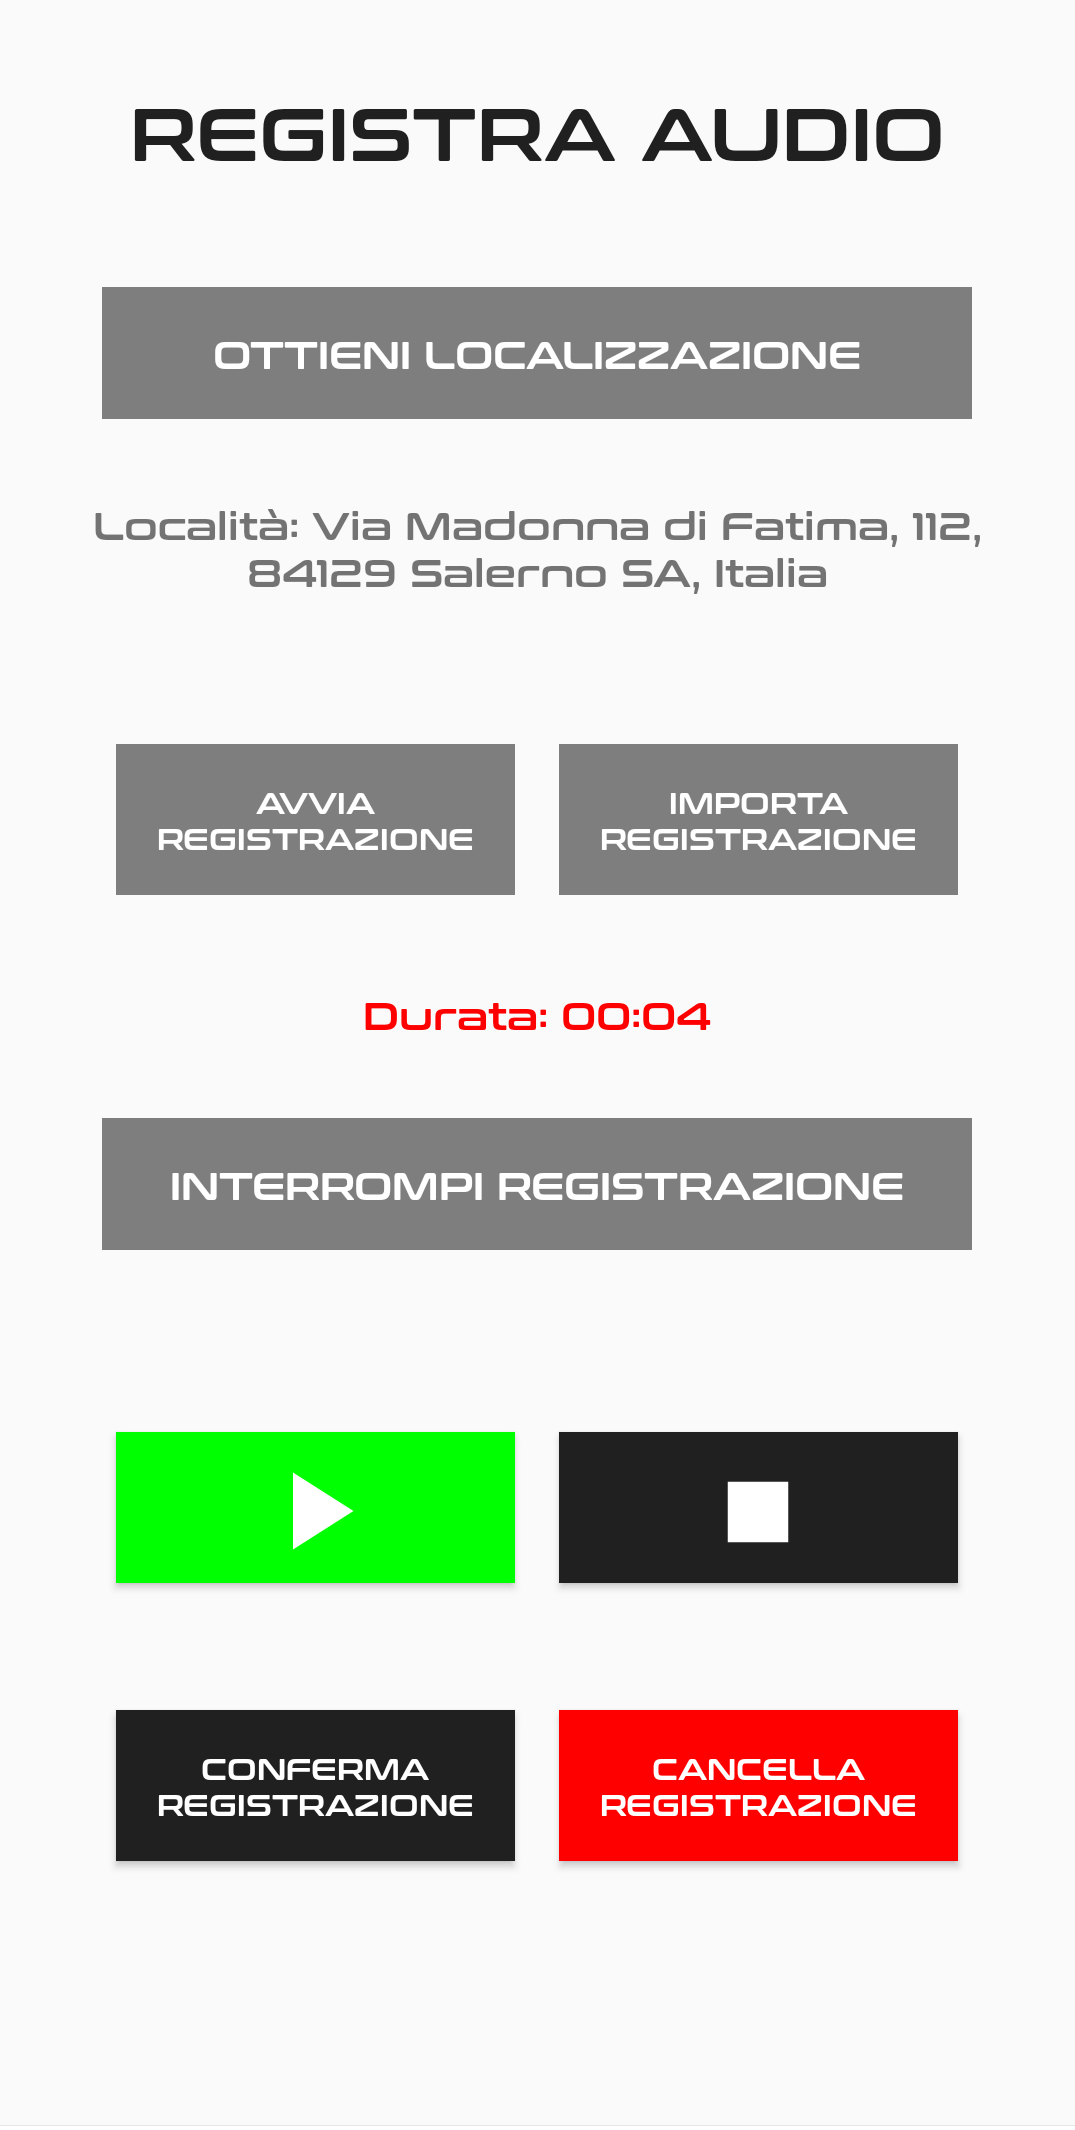
\includegraphics[width=0.8\textwidth]{registrazioneaudio.png}\vspace*{40pt}
\end{minipage}
\begin{minipage}[t]{0.35\textwidth}
    \centering
    \vspace*{20pt}
    
\includegraphics[width=0.8\textwidth]{uploadlist.png}
\end{minipage}
\hfill
\begin{minipage}[t]{0.6\textwidth}
    \raggedright
    \vspace*{20pt}
    Gli audio salvati per essere caricati successivamente sono presenti in questa Activity, visibili all'interno di una Recycler View.\\
    Qui è possibile avviare manualmente il caricamento, anche con dati mobili. Verrà mostrato lo stesso \textit{Alert Dialog} mostrato nella fase di registrazione. In caso di connessione Wi-Fi, il caricamento avverrà senza mostrare alcun pop-up.\vspace*{14pt}\\
    \textit{Nota Bene}: vedremo successivamente come gli audio verranno caricati automaticamente in background in caso di connessione Wi-Fi.\vspace*{14pt}\\
    Un altro dettaglio è inerente all'audio registrato. Il formato audio registrato tramite la classe \textbf{MediaRecorder} di Android non è supportato nativamente dal server. Viene quindi utilizzata la libreria \textbf{ffmpeg} per gestire la conversione del file audio in un formato supportato.
\end{minipage}

\quad \vspace*{10pt}\\
\textit{Mappa}\\
\begin{minipage}[t]{0.6\textwidth}
    \raggedright
    \vspace*{20pt}
    Il pulsante \textbf{Mappa} nella Navigation Bottom Bar permette di caricare il fragment inerente alla mappa. Sulla mappa sono presenti tutti gli audio della chiamata API \textit{"audio/all"}.\\
    Per la mappa viene utilizzata la libreria \textbf{osmdroid}, alternativa gratuita a Google Maps.\vspace*{14pt}\\
    Il Fragment presenta inoltre due Floating Button. Uno per ottenere l'intero elenco degli audio in piattaforma sotto forma di lista (se ne parlerà successivamente nella sezione Extra).\\
    L'altro per ottenere la localizzazione e zoommare sulla mappa nel punto in cui ci troviamo. Vengono inoltre richiesti i permessi per la localizzazione la prima volta.
\end{minipage}
\hfill
\begin{minipage}[t]{0.35\textwidth}
    \centering
    \vspace*{10pt}
    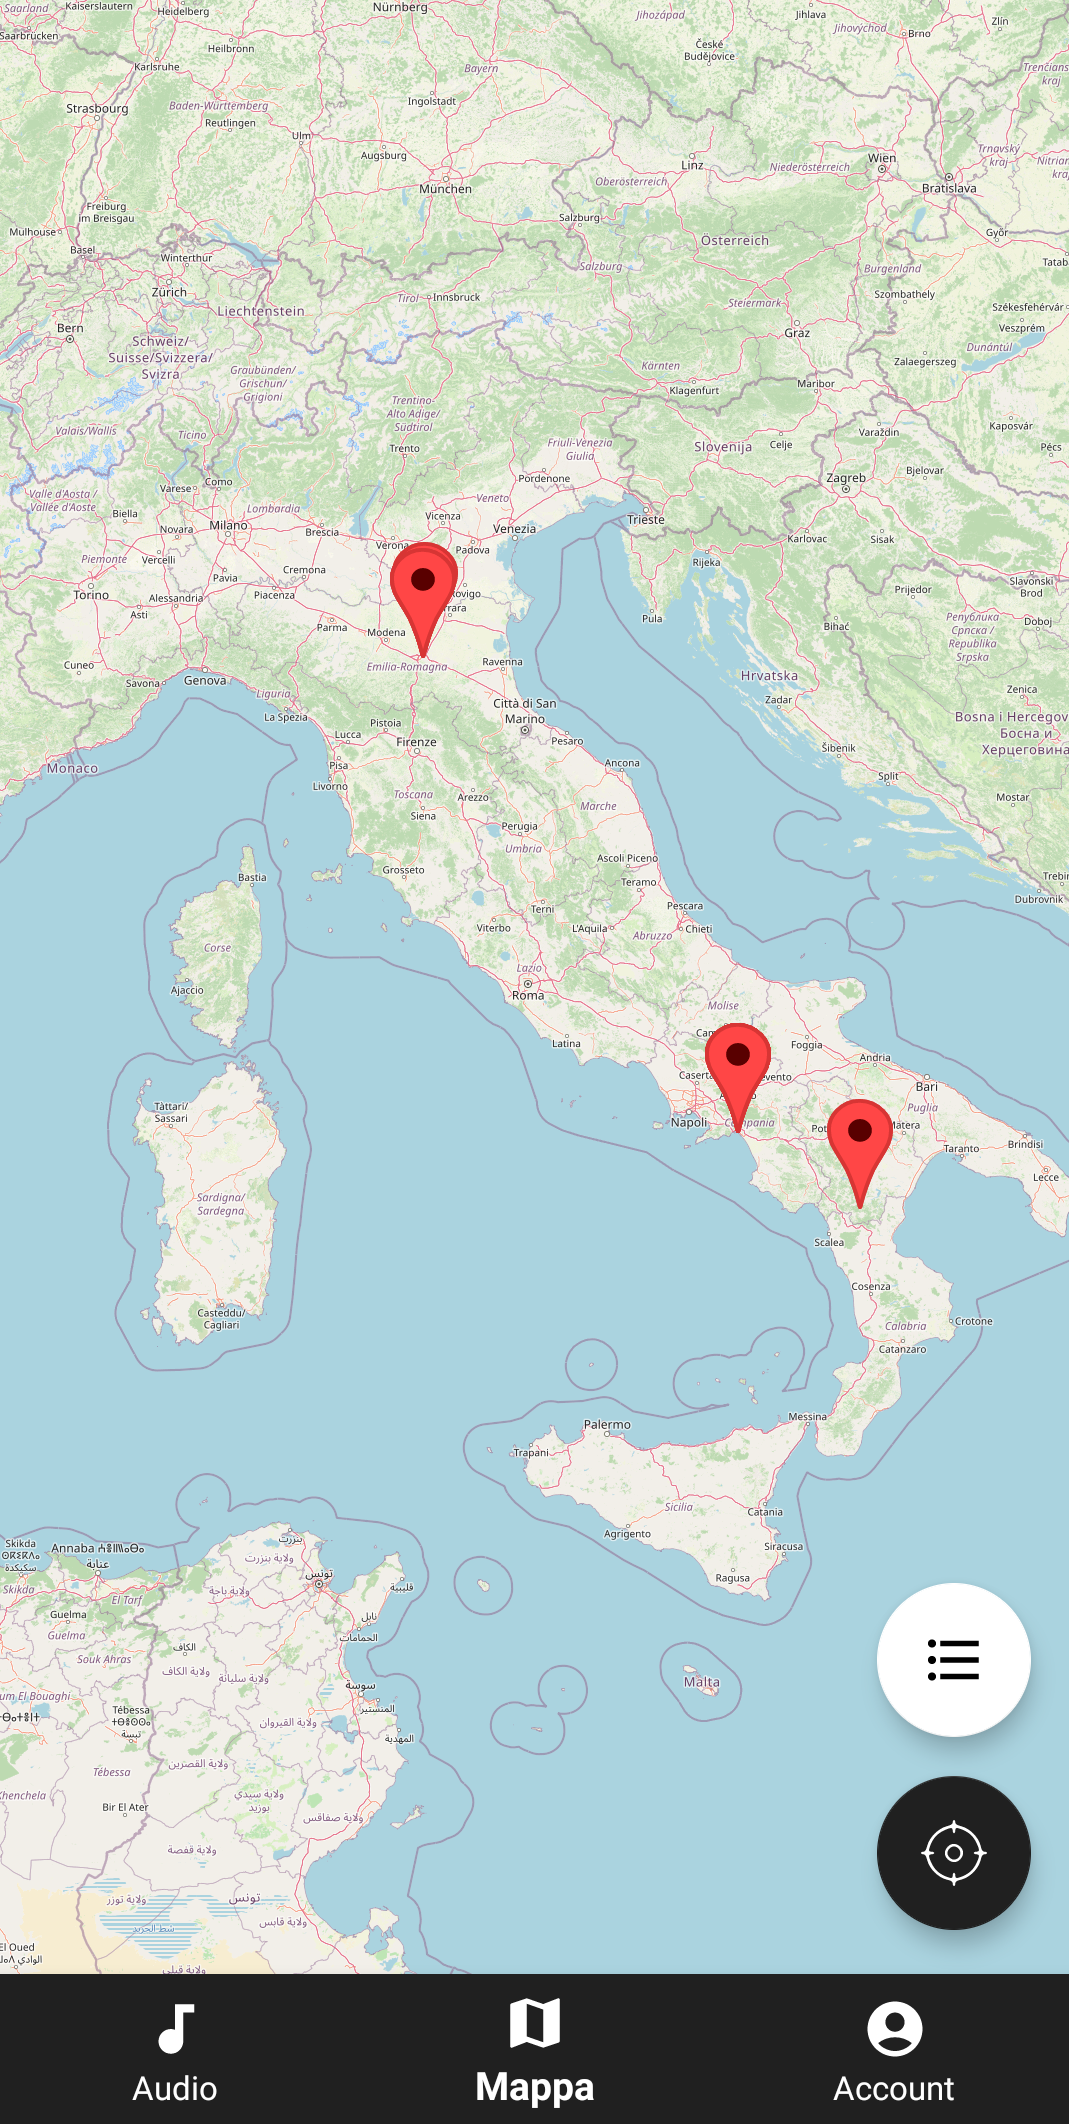
\includegraphics[width=0.8\textwidth]{mappa.png}\vspace*{40pt}
\end{minipage}
\begin{minipage}[t]{0.35\textwidth}
    \centering
    \vspace*{20pt}
    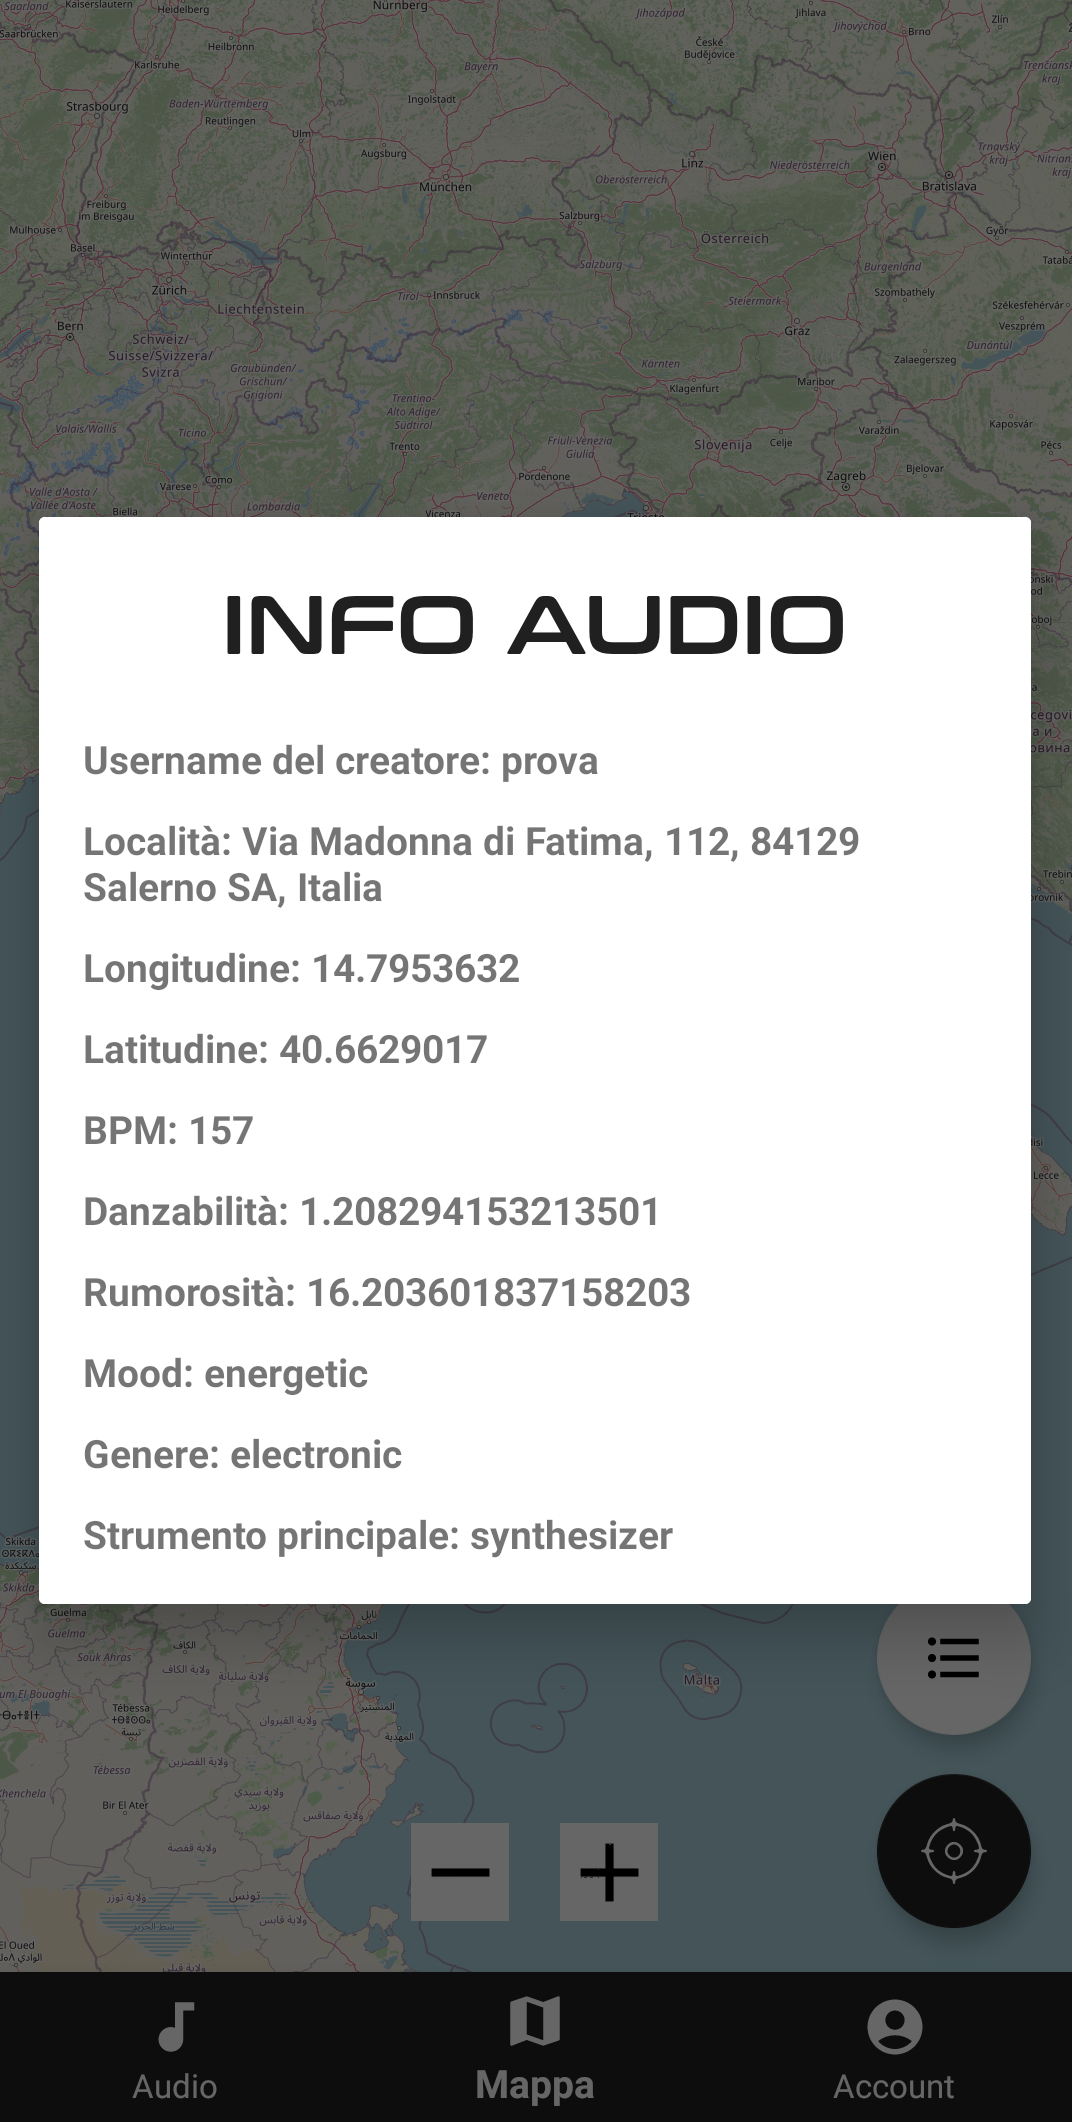
\includegraphics[width=0.8\textwidth]{audiodatadialog.png}
\end{minipage}
\hfill
\begin{minipage}[t]{0.6\textwidth}
    \raggedright
    \vspace*{30pt}
    Una volta premuto su uno dei \textit{marker} presenti sulla mappa, verrà aperto un \textbf{DialogFragment} custom. All'interno di questo Fragment si possono osservare tutti i metadati inerenti all'audio selezionato.\\
    Anche in questo caso, viene controllata la presenza dei metadati dell'audio nel database locale. In caso negativo, viene effettuata la chiamata API \textit{"audio/\{id\}"} per ottenere e salvare i metadati.\vspace*{14pt}\\
    Una funzionalità extra, della quale parleremo successivamente, effettua un \textbf{fetching automatico} se sullo schermo sono presenti dieci o meno marker. In questo modo non ci sarà alcun delay durante l'apertura del DialogFragment, avendo già i metadati salvati in locale.
\end{minipage}

\quad \vspace*{20pt}\\
\textit{Account}\\
\begin{minipage}[t]{0.6\textwidth}
    \raggedright
    \vspace*{20pt}
    L'ultimo Fragment accessibile tramite la Navigation Bottom Bar è quello inerente all'\textbf{Account}.\\
    In questa schermata è presente una breve descrizione dell'applicativo.\vspace*{14pt}\\
    Vengono inoltre mostrati due bottoni.\\
    Uno per effettuare il \textbf{Logout}, tornando all'Activity Login.\\
    L'altro, invece, per \textbf{cancellare il proprio account}, effettuando la chiamata API \textit{"auth/unsubscribe"}.
\end{minipage}
\hfill
\begin{minipage}[t]{0.35\textwidth}
    \centering
    \vspace*{10pt}
    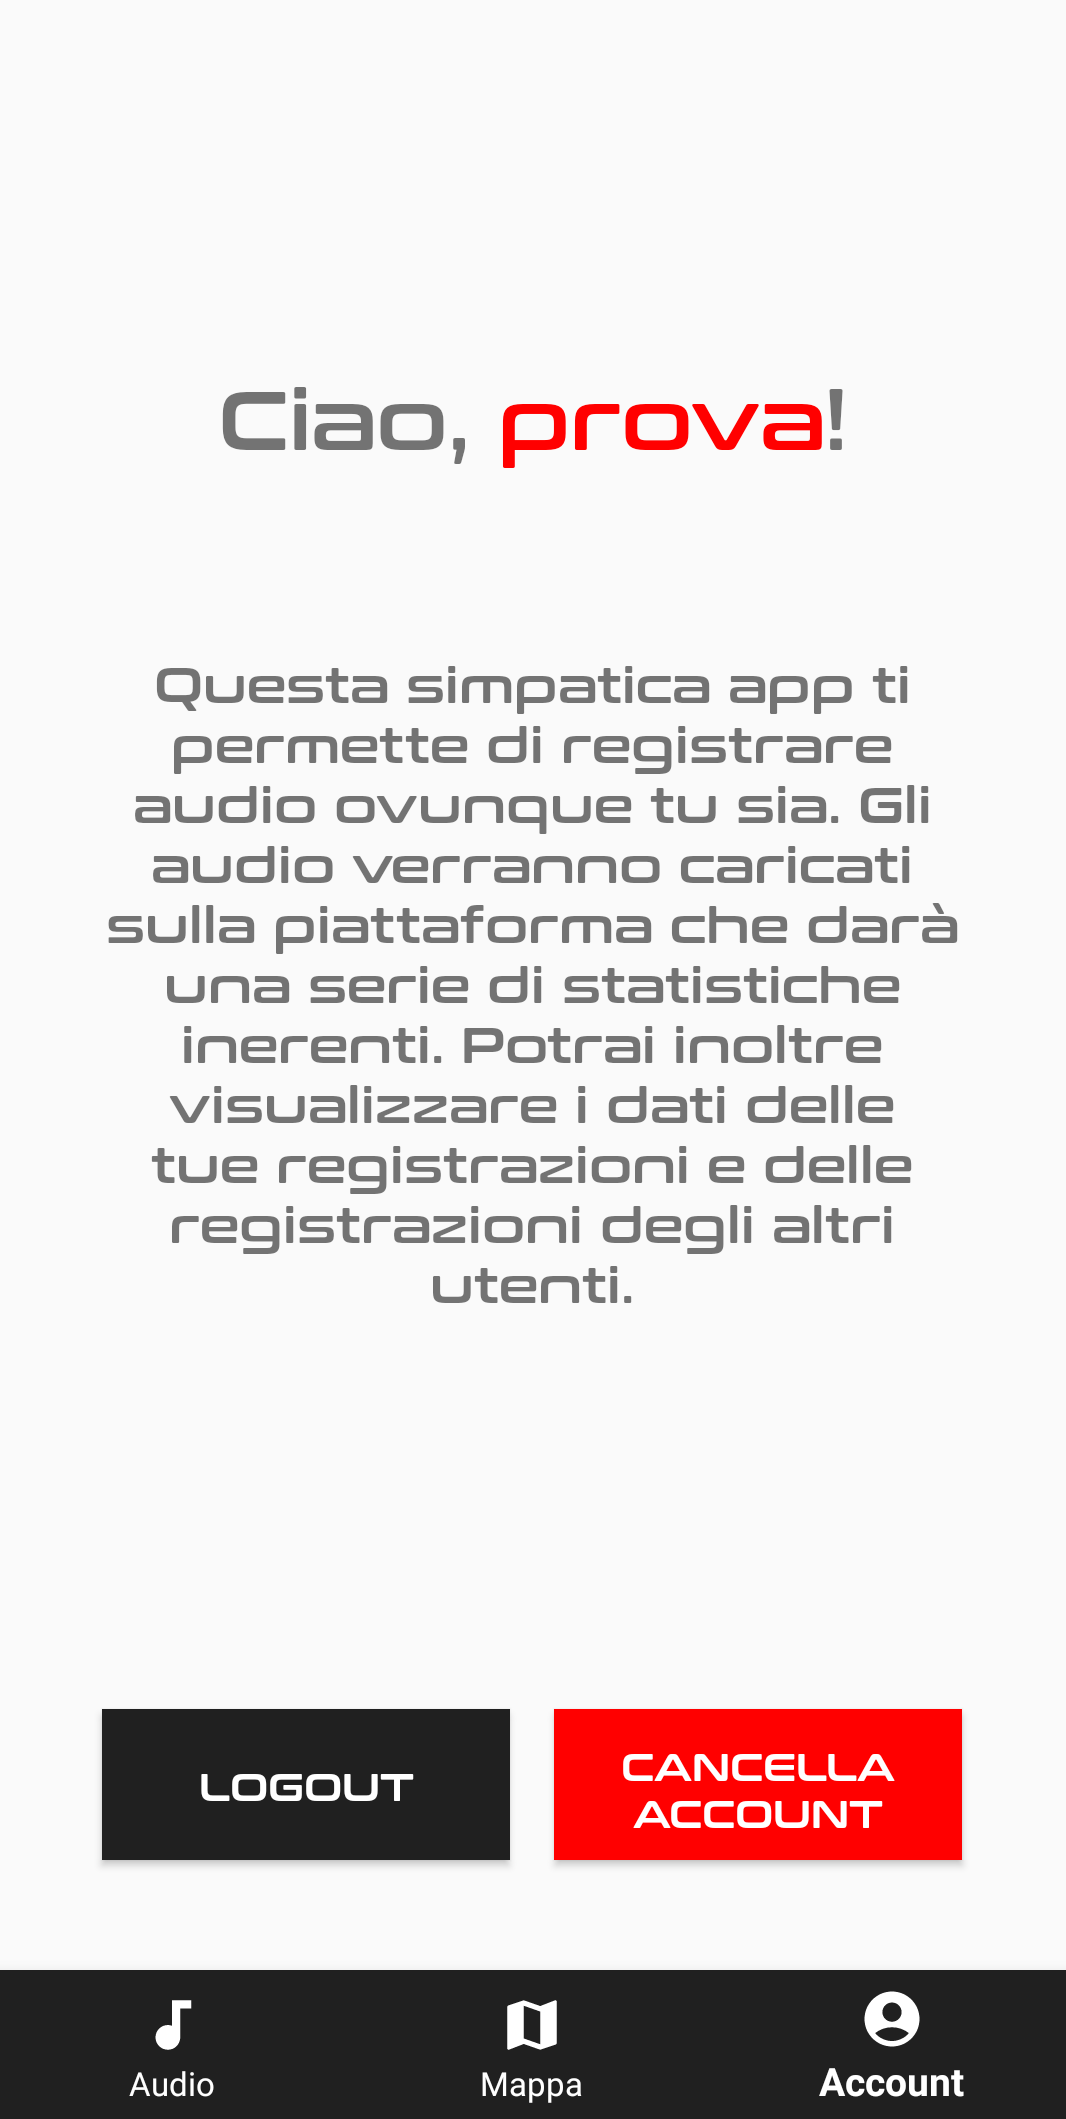
\includegraphics[width=0.8\textwidth]{account.png}\vspace*{40pt}
\end{minipage}
\textit{Servizio in Background}\\
Come richiesto dalla traccia, è stato implementato un \textbf{servizio che agisce in background}.\\
Il \textbf{Service} in questione controlla ogni cambiamento della connessione Wi-Fi, e grazie ad un \textbf{Broadcast Receiver} ogni cambiamento viene ascoltato e gestito. In caso di connessione Wi-Fi stabile e connessa ad Internet, verrà controllato l'elenco degli upload in attesa. Se l'elenco risulta vuoto, non verrà eseguita alcuna funzione. In caso contrario, tutti gli upload presenti verranno caricati sul server, salvando il risultato nel database locale per utilizzi futuri.\\
Concluso l'upload, verrà avviato un \textbf{Worker}, il quale si occupa di \textbf{inviare la notifica} all'utente.\\
\begin{center}
    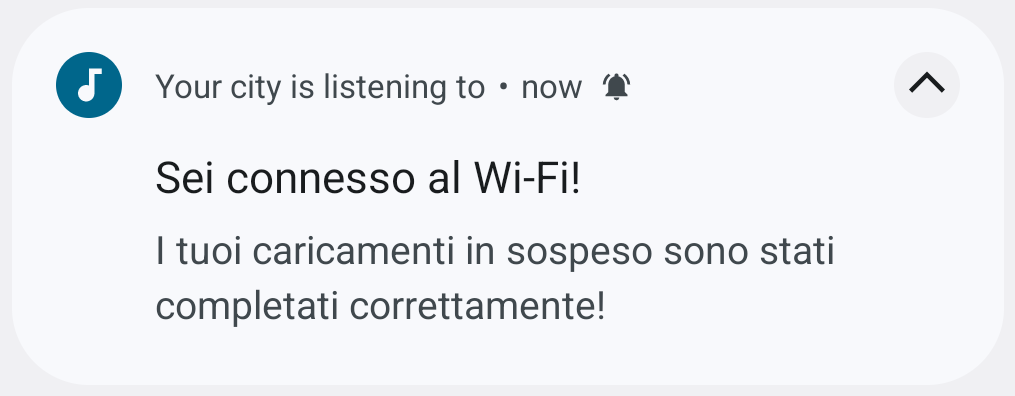
\includegraphics[width=0.6\textwidth]{notifica.png}
\end{center}
Premendo sulla notifica, verrà aperta l'app, permettendo di interagire con gli audio caricati.

\quad \vspace*{10pt}\\
\textit{Sezione Offline}\\
\begin{minipage}[t]{0.6\textwidth}
    \raggedright
    \vspace*{10pt}
    Si accede alla \textbf{sezione Offline} se si apre l'app senza connessione, o se durante l'utilizzo dell'app non è piu disponibile una connessione ad Internet.\\
    In questa sezione l'Activity principale propone funzionalità limitate. Il Fragment della Mappa e dell'Account non offrono alcuna funzionalità, dipendendo da Internet (Mappa) e da un account specifico (Account).\\
    L'implementazione della sezione Offline si basa su una logica indipendente da un singolo account.\vspace*{14pt}\\
    Nella sezione Audio Personali sarà possibile consultare tutti gli audio salvati all'interno del database locale.\\
    Anche in questo caso, la visualizzazione dei singoli audio avviene tramite Recycler View.
\end{minipage}
\hfill
\begin{minipage}[t]{0.35\textwidth}
    \centering
    \vspace*{0pt}
    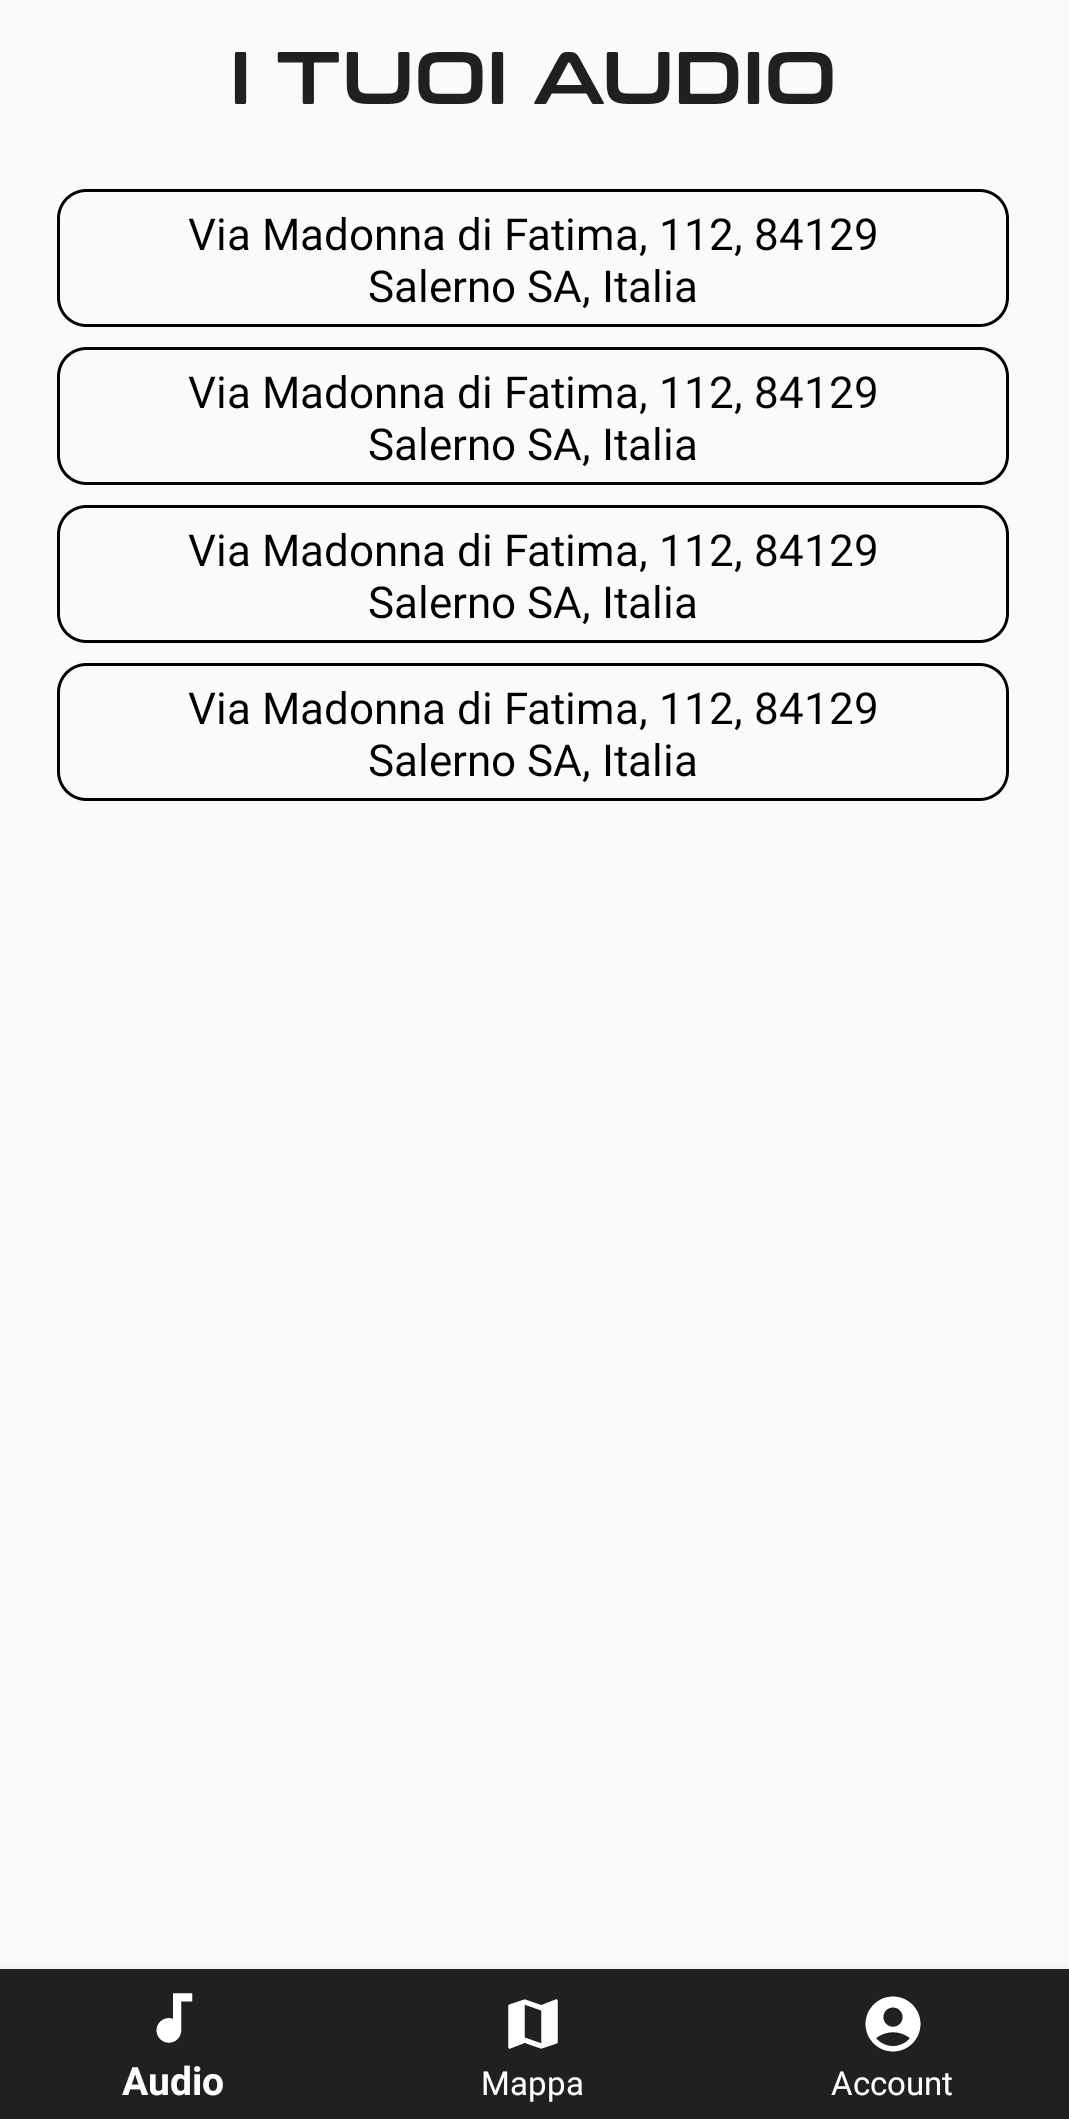
\includegraphics[width=0.8\textwidth]{offlinelist.png}\vspace*{40pt}
\end{minipage}
\begin{minipage}[t]{0.35\textwidth}
    \centering
    \vspace*{0pt}
    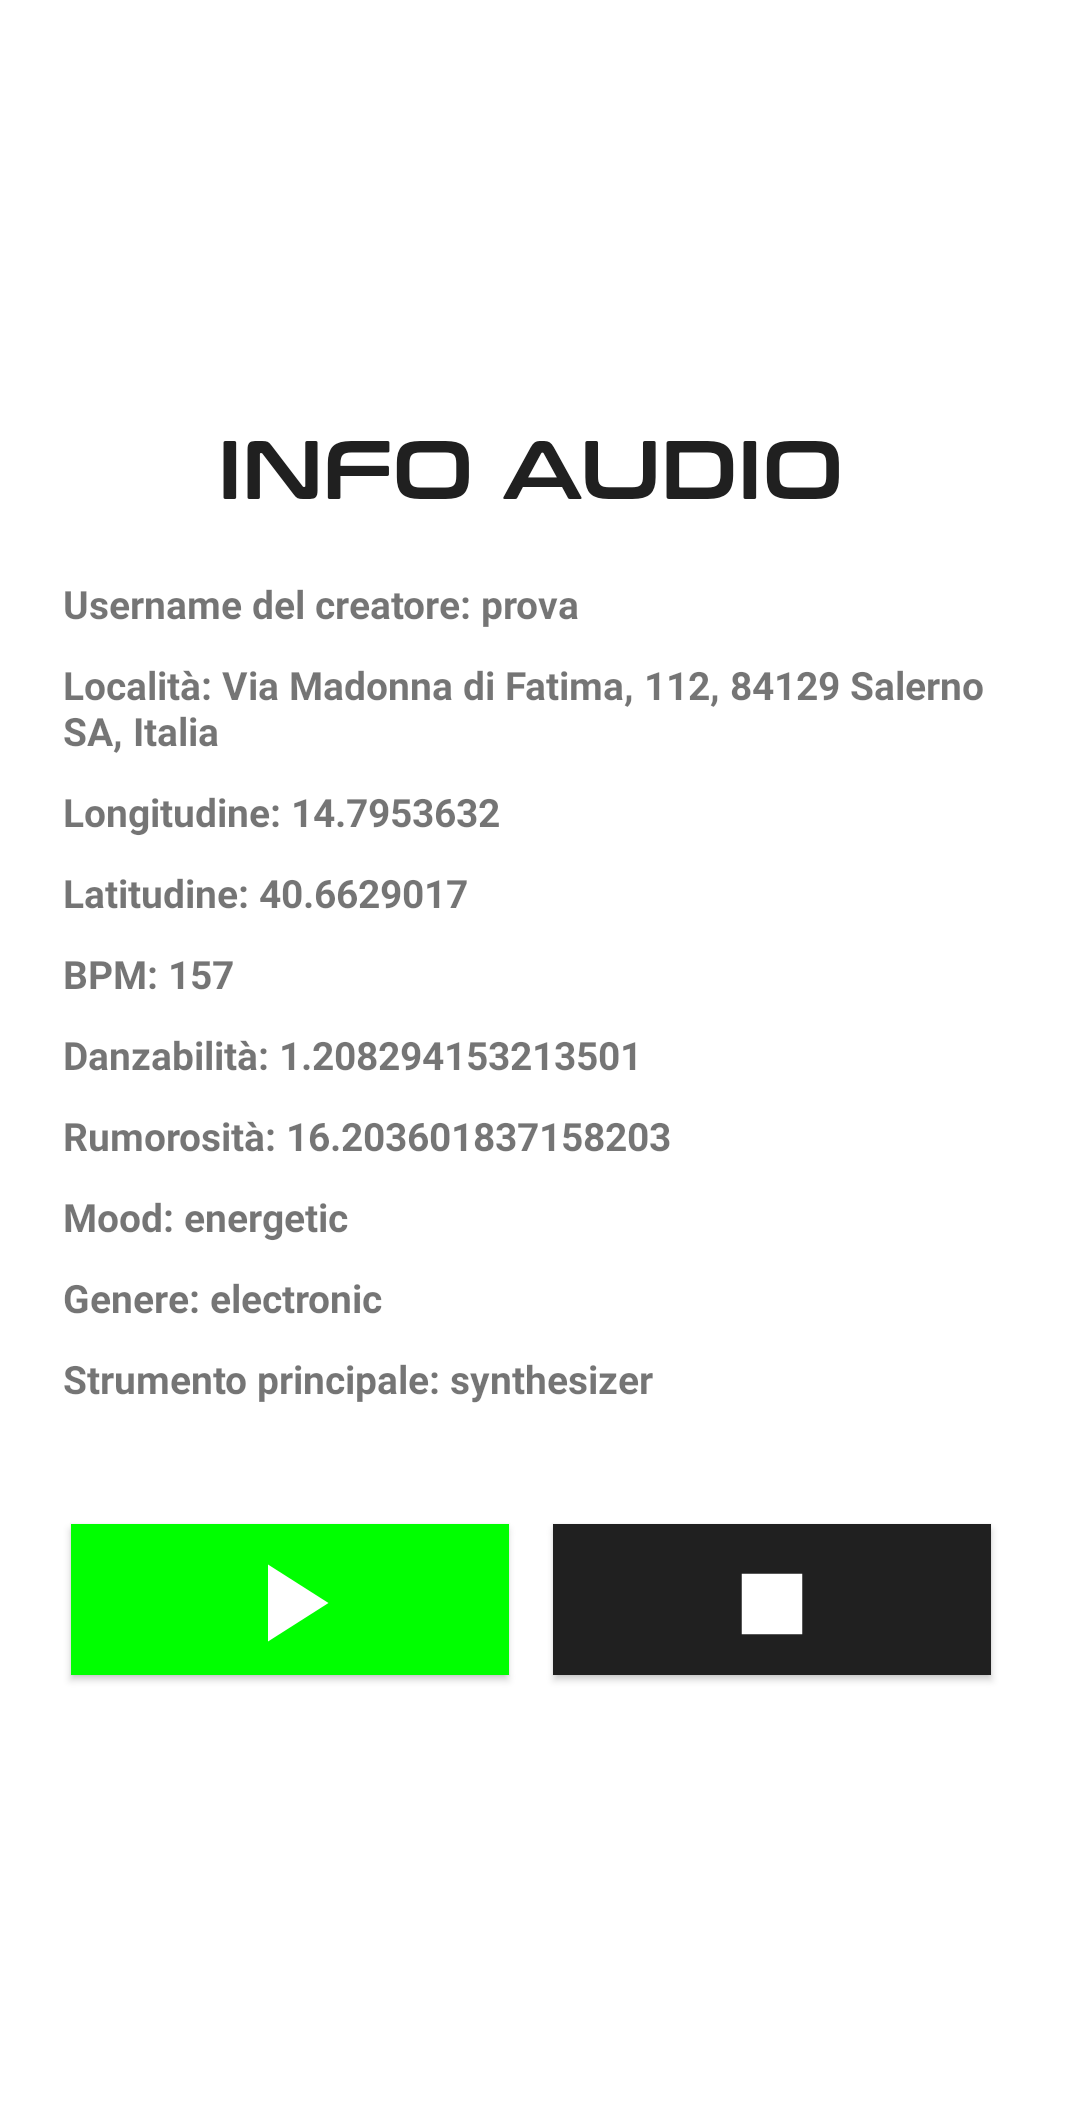
\includegraphics[width=0.8\textwidth]{offlineaudiodata.png}
\end{minipage}
\hfill
\begin{minipage}[t]{0.6\textwidth}
    \raggedright
    \vspace*{50pt}
    Una volta premuto su l'elemento scelto, verrà aperta un'Activity molto simile alla sua controparte \textit{"Online"}, privata di alcune funzionalità dipendenti dal server.\vspace*{14pt}\\
    Sarà ovviamente ancora possibile ascoltare l'audio, essendo salvato in memoria e non sul server.\vspace*{14pt}\\
    Per tornare alla versione completa dell'applicativo, bisognerà chiudere a riaprire l'app una volta stabilita una connessione ad Internet.
\end{minipage}

\pagebreak

\subsection*{Funzionalità Extra}
\large

Come anticipato, sono state aggiunte \textbf{funzionalità extra} all'interno dell'app. Alcune di queste sono richieste opzionali presenti nella traccia, altre sono funzionalità aggiunte in autonomia.\vspace*{14pt}\\
\textbf{Importa audio}\\
Una funzionalità che può risultare comoda in molti casi è l'\textbf{importare audio} dall'esterno. Come visto in precedenza nell'Activity inerente alla \textit{registrazione audio}, è presente un bottone che permette di importare audio dalla propria memoria.\\
Questa funzione è realizzata tramite un \textit{Intent} di tipo \textit{"audio/*"}, il quale permette di selezionare soltanto file audio. Una volta selezionato, la libreria \textit{ffmpeg} procederà a convertire e salvare l'audio in memoria, rendendolo fruibile all'interno dell'app.
\vspace*{14pt}\\
\textbf{Salvataggio in locale}\\
Come consigliato dalla traccia, i metadati inerenti agli audio vengono salvati in locale, all'interno di un database, per essere riutilizzati successivamente.\\
Questo procedimento avviene sia per gli audio caricati dall'utente -- denominati \textit{MyAudio} -- sia per gli audio presenti in piattaforma -- denominati \textit{AllAudio}.\vspace*{14pt}\\
Il salvataggio in locale dei metadati permette all'applicativo di non dover interrogare il server per ogni richiesta effettuata dall'utente. Prima di interpellare il server, verrà controllata la presenza dei metadati in locale. Se non presenti, verrà effettuata la chiamata API al server, con conseguente salvataggio in locale della risposta ottenuta.\vspace*{14pt}\\
\textbf{Upload in background}\\
Anche in questo caso, viene aggiunta una funzionalità extra alla richiesta della traccia.\\
L'app non invia una notifica quando una connessione Wi-Fi stabile è presente, ma prosegue in automatico con l'upload in background, inviando una notifica al termine dell'upload.\vspace*{14pt}\\
Come spiegato in precedenza, il tutto avviene grazie ad un \textbf{Service}, il quale controla in background ogni cambiamento della connessione Wi-Fi grazie ad un \textbf{Broadcast Receiver}. Una volta stabilita la connessione Wi-Fi stabile, verrà controllata la presenza di upload in attesa di essere caricati. Se presenti, il Service procederà all'upload in background, inviando la notifica al termine dell'operazione.\vspace*{14pt}\\
\textbf{Fetching automatico AllAudio}\\
Per rendere l'esperienza più fluida, è stato implementato un \textbf{fetching automatico} per gli AllAudio visibili sulla mappa.\\
Ogni volta che avviene un movimento sulla mappa, un controllo sul numero dei marker visibili viene effettuato (\textit{Nota Bene: è presente un debounce di 7 secondi tra i controlli}). Se il numero è minore o uguale a 10, avviene un \textit{fetching automatico} dei metadati dei marker visibili a schermo, permettendo una visualizzazione più rapida del DialogFragment.\\
Il fetching salva in automatico all'interno del database locale tutti i metadati ottenuti, utilizzandoli per tutte le richieste successive.\vspace*{14pt}\\
\pagebreak
\quad \vspace*{0pt}\\
\textbf{Lista di AllAudio}\\
\begin{minipage}[t]{0.6\textwidth}
    \raggedright
    \vspace*{20pt}
    Oltre alla visualizzazione sulla mappa dei diversi \textit{marker} inerenti ad un singolo audio, è stata aggiunta una nuova visualizzazione sotto forma di lista. Anche in questo caso, come per le liste presenti in tutta l'app, è stata usata una Recycler View.\vspace*{14pt}\\
    Premendo su un elemento verrà aperto il DialogFragment custom utilizzato anche per il click sui marker.
\end{minipage}
\hfill
\begin{minipage}[t]{0.35\textwidth}
    \centering
    \vspace*{0pt}
    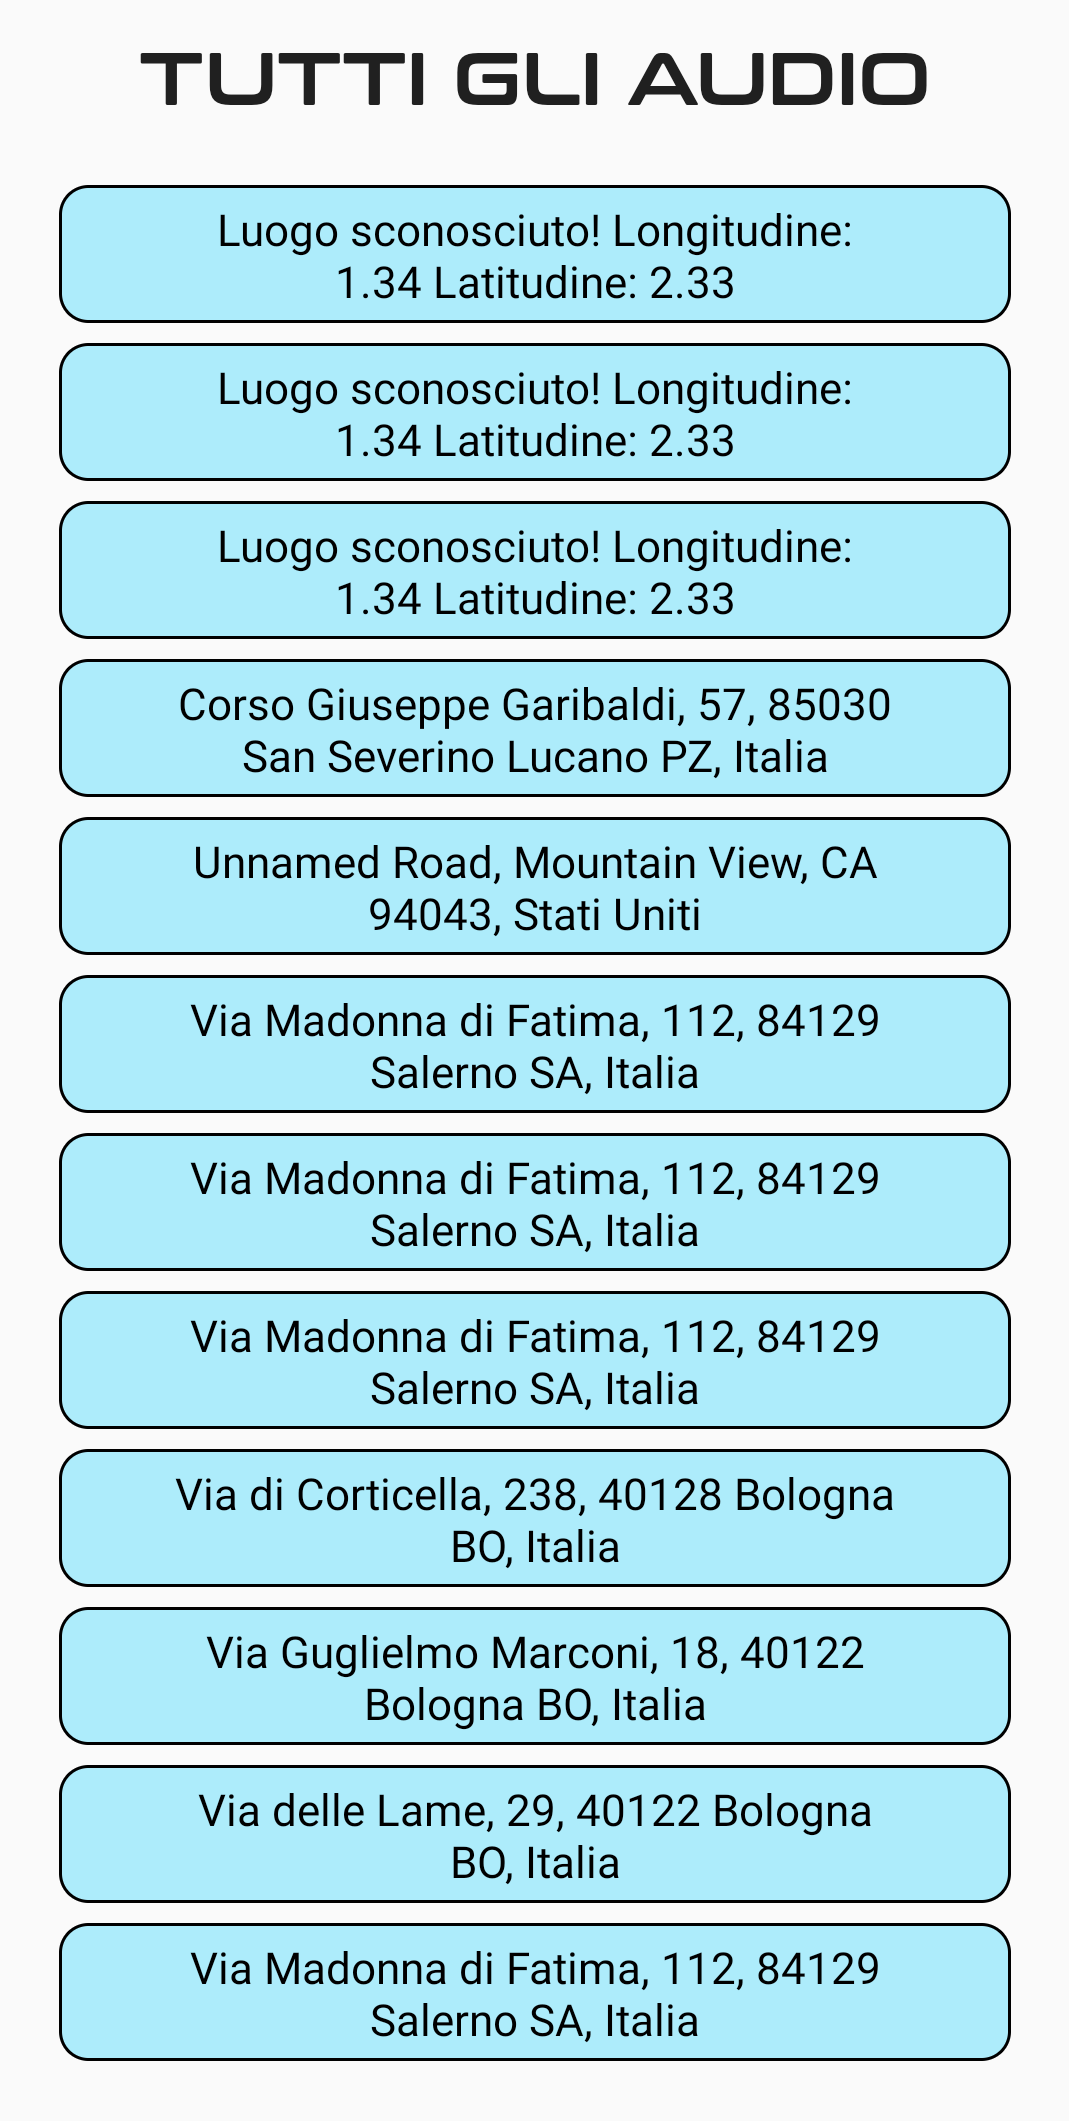
\includegraphics[width=0.62\textwidth]{allaudiolist.png}\vspace*{40pt}
\end{minipage}
\end{document}